\chapter{HASIL DAN PEMBAHASAN}

\section{Pemeriksaan Perangkat Lunak}
Penelitian ini membandingkan kinerja Hadoop dan Spark pada \textit{platform cloud} DigitalOcean menggunakan alat pengujian data besar yang bernama HiBench pada lingkup \textit{Micro Benchmarks}, yaitu \textit{Word Count} dan \textit{Sort} dengan data masukan berupa teks yang dibuat oleh \textit{data generation} pada tahap persiapan. 

Sebelum memulai eksperimen, serangkaian pemeriksaan dilakukan untuk memastikan bahwa semua perangkat lunak yang terlibat berfungsi dengan baik. Tahapan ini penting untuk menjamin validitas hasil penelitian. Berikut adalah pemeriksaan yang dilakukan, yaitu
\begin{enumerate}
	\item \textbf{Pengecekan versi Hadoop}. Versi Hadoop yang digunakan dalam penelitian ini adalah 2.4.0. Verifikasi versi dilakukan melalui perintah \textit{hadoop version}, seperti yang ditunjukkan pada Gambar \ref{fig:versi-hadoop}. 
		\begin{figure}[h]
		    \centering
		    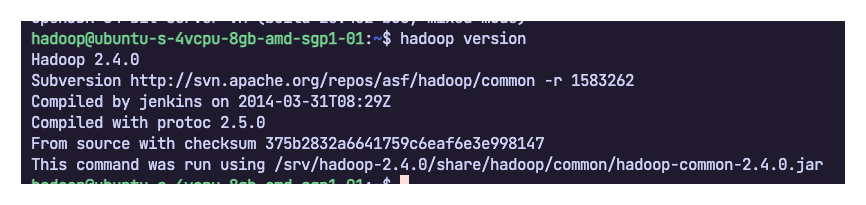
\includegraphics[width=0.8\textwidth]{figures/ch04/versi-hadoop}
		    \caption{Pengecekan Versi Hadoop}
		    \label{fig:versi-hadoop}
		\end{figure}
	\item \textbf{Pengecekan versi Spark}. Versi Spark yang digunakan adalah 2.1.3. Verifikasi dilakukan dengan perintah \textit{spark-submit --version}, seperti yang ditunjukkan pada Gambar \ref{fig:versi-spark}.
		\begin{figure}[h]
		    \centering
		    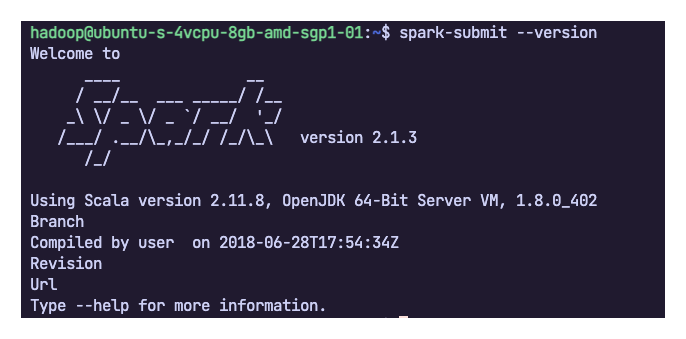
\includegraphics[width=0.8\textwidth]{figures/ch04/versi-spark}
		    \caption{Pengecekan Versi Spark}
		    \label{fig:versi-spark}
		\end{figure}
	\item \textbf{Pemeriksaan \textit{service} yang berjalan ketika beban kerja belum dijalankan}. Status layanan (\textit{services}) yang berjalan pada komputer diperiksa dalam keadaan tanpa beban kerja (\textit{idle}). Layanan yang diharapkan aktif meliputi: Jps, ResourceManager, DataNode, NodeManager, NameNode, dan SecondaryNameNode. Gambar \ref{fig:service-dasar} menunjukkan hasil pemeriksaan layanan dasar.		
		\begin{figure}[h]
		    \centering
		    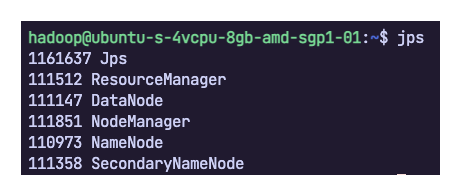
\includegraphics[width=0.9\textwidth]{figures/ch04/service-dasar}
		    \caption{Pengecekan \textit{Service} yang Berjalan (Normal)}
		    \label{fig:service-dasar}
		\end{figure}
	\item \textbf{Pemeriksaan \textit{service} yang berjalan ketika menggunakan Hadoop}. Ketika beban kerja Hadoop dijalankan, layanan tambahan seperti YarnChild, MRAppMaster, dan RunJar  diharapkan aktif, di samping layanan dasar yang telah disebutkan. Gambar \ref{fig:service-hadoop} menunjukkan hasil pemeriksaan layanan saat Hadoop aktif.
		\begin{figure}[h]
		    \centering
		    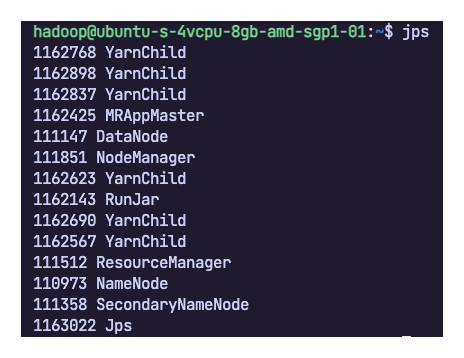
\includegraphics[width=0.8\textwidth]{figures/ch04/service-hadoop}
		    \caption{Pengecekan \textit{Service} yang Berjalan (Hadoop)}
		    \label{fig:service-hadoop}
		\end{figure}
	\item \textbf{Pemeriksaan \textit{service} yang berjalan ketika menggunakan Spark}. Ketika beban kerja Spark dijalankan, layanan seperti CoarseGrainedExecutorBackend, ExecutorLauncher, dan SparkSubmit diharapkan aktif, di samping layanan dasar.  Gambar \ref{fig:service-spark} menunjukkan hasil pemeriksaan layanan saat Spark aktif.
		\begin{figure}[h]
		    \centering
		    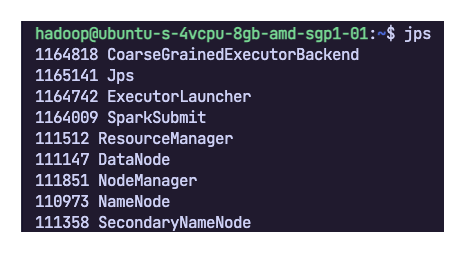
\includegraphics[width=0.9\textwidth]{figures/ch04/service-spark}
		    \caption{Pengecekan \textit{Service} yang Berjalan (Spark)}
		    \label{fig:service-spark}
		\end{figure}
\end{enumerate}

\section{Parameter yang Digunakan}
Selama pengujian, beberapa parameter pada HiBench, Hadoop, dan Spark dikonfigurasi secara tetap untuk menjaga konsistensi dan memungkinkan perbandingan yang adil. Tabel \ref{table:conf-hibench} dan \ref{table:conf-spark} merangkum konfigurasi parameter yang digunakan.

\begin{table}[h]
\caption{Konfigurasi HiBench}
\label{table:conf-hibench}
\centering
\begin{tabular}{ll}
\hline
\multicolumn{1}{c}{\textbf{Nama Parameter}}  & \multicolumn{1}{c}{\textbf{Nilai}} \\ \hline
hibench.default.map.parallelism     & 8                         \\
hibench.default.shuffle.parallelism & 8 \\ \hline                        
\end{tabular}
\end{table}

\begin{table}[h]
\caption{Konfigurasi Spark}
\label{table:conf-spark}
\centering
\begin{tabular}{ll}
\hline
\multicolumn{1}{c}{\textbf{Nama Parameter}}  & \multicolumn{1}{c}{\textbf{Nilai}} \\ \hline
hibench.yarn.executor.num     & 2                         \\
hibench.yarn.executor.cores & 4 \\ 
spark.executor.memory   & 4G \\
spark.driver.memory & 4G \\ \hline                        
\end{tabular}
\end{table}

\newpage
Parameter \textit{hibench.default.map.parallelism} memiliki peran yang berbeda pada Hadoop dan Spark. Pada Hadoop, parameter ini menentukan jumlah \textit{Mapper}, yaitu proses yang bertanggung jawab untuk memproses data secara paralel pada tahap \textit{Map}. Pada Spark, parameter ini menentukan jumlah partisi data, yaitu unit pemrosesan dasar dalam Spark.

Parameter \textit{hibench.default.shuffle.parallelism} juga memiliki peran yang berbeda pada Hadoop dan Spark. Pada Hadoop, parameter ini menentukan jumlah \textit{Reducer}, yaitu proses yang bertanggung jawab untuk menggabungkan hasil dari tahap \textit{Map}. Pada Spark, parameter ini menentukan jumlah \textit{Shuffle partition}, yaitu jumlah partisi data yang digunakan selama tahap \textit{Shuffle}, yaitu proses pengocokan dan pengurutan data antara tahap \textit{Map} dan \textit{Reduce}.

Berikut penjelasan mengenai parameter Spark pada Tabel \ref{table:conf-spark}:
\begin{enumerate}
	\item \textbf{hibench.yarn.executor.num}: Parameter ini menentukan jumlah \textit{executor} yang akan dialokasikan untuk aplikasi Spark. \textit{Executor} adalah proses yang berjalan pada node pekerja (\textit{worker node}) di kluster YARN dan bertanggung jawab untuk menjalankan task Spark.
	\item \textbf{hibench.yarn.executor.cores}: Parameter ini menentukan jumlah core CPU yang dialokasikan untuk setiap \textit{executor}. Semakin banyak core yang dialokasikan, semakin banyak task yang dapat dijalankan secara paralel oleh setiap \textit{executor}.
	\item \textbf{spark.executor.memory}: Parameter ini menentukan jumlah memori yang dialokasikan untuk setiap \textit{executor}. Memori ini digunakan untuk menyimpan data yang diproses oleh \textit{executor}, seperti RDD dan data yang di-\textit{cache}.
	\item \textbf{spark.driver.memory}: Parameter ini menentukan jumlah memori yang dialokasikan untuk proses driver Spark. Driver bertanggung jawab untuk mengelola aplikasi Spark, menjadwalkan task, dan mengumpulkan hasil.
\end{enumerate}

\section{Data Keluaran yang Dihasilkan}

Setiap pengujian akan menghasilkan berkas output berupa data HiBench \textit{Report} dan Dool \textit{System Monitoring}. Data HiBench \textit{Report} akan terlihat seperti pada Gambar \ref{fig:data-hibench-report}. Pada Gambar tersebut, terlihat bahwa ekstensi berkasnya \textit{.report} dan terlihat beberapa data seperti jenis beban kerja, aplikasi yang digunakan, besar input data, durasi, dan \textit{throughput}.

\begin{figure}[h]
    \centering
    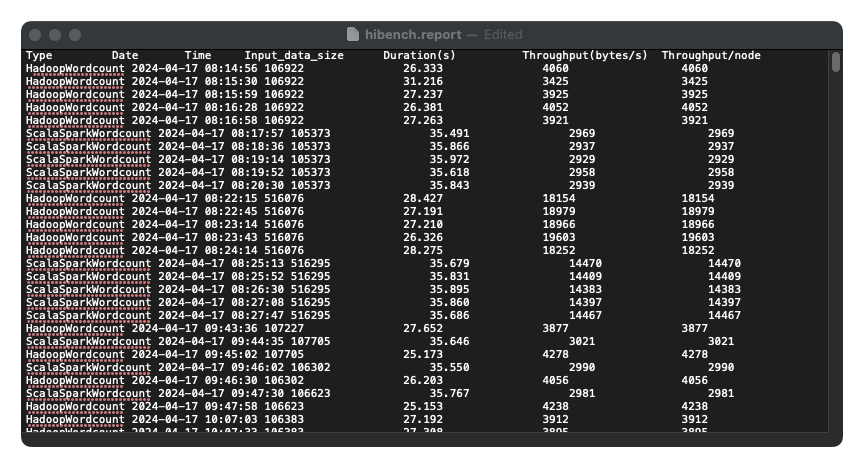
\includegraphics[width=1\textwidth]{figures/ch04/data-hibench}
    \caption{Data HiBench \textit{Report}}
    \label{fig:data-hibench-report}
\end{figure}

Dool, alat monitoring sistem, menghasilkan berkas CSV (\textit{comma-separated value}) untuk setiap perulangan eksperimen. Dengan demikian, terdapat sekitar 240 berkas CSV, seperti yang ditunjukkan pada Gambar \ref{fig:data-dool-luar}. Penamaan berkas mengikuti format: [jenis beban kerja]-[ukuran data]-[nomor perulangan]-[aplikasi]. Sebagai contoh, \textit{sort-fivegig-1-hadoop.csv} menunjukkan \textit{data monitoring} untuk beban kerja sort, data masukan 5 GB, perulangan pertama, dan aplikasi Hadoop.

\begin{figure}[h]
    \centering
    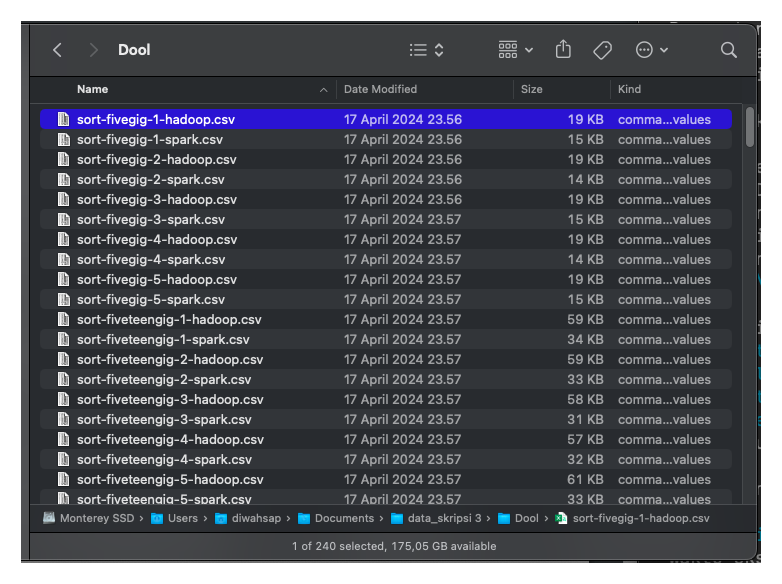
\includegraphics[width=0.7\textwidth]{figures/ch04/data-dool-luar}
    \caption{Berkas Dool}
    \label{fig:data-dool-luar}
\end{figure}

Struktur data Dool, yang ditunjukkan pada Gambar \ref{fig:data-dool-dalam}, mencakup baris \textit{header} (baris 1-4) dan nama kolom (baris 6). Data ini akan dianalisis lebih lanjut untuk mendapatkan \textit{insight} tentang kinerja Hadoop dan Spark.

\begin{landscape}
\begin{figure}[h]
    \centering
    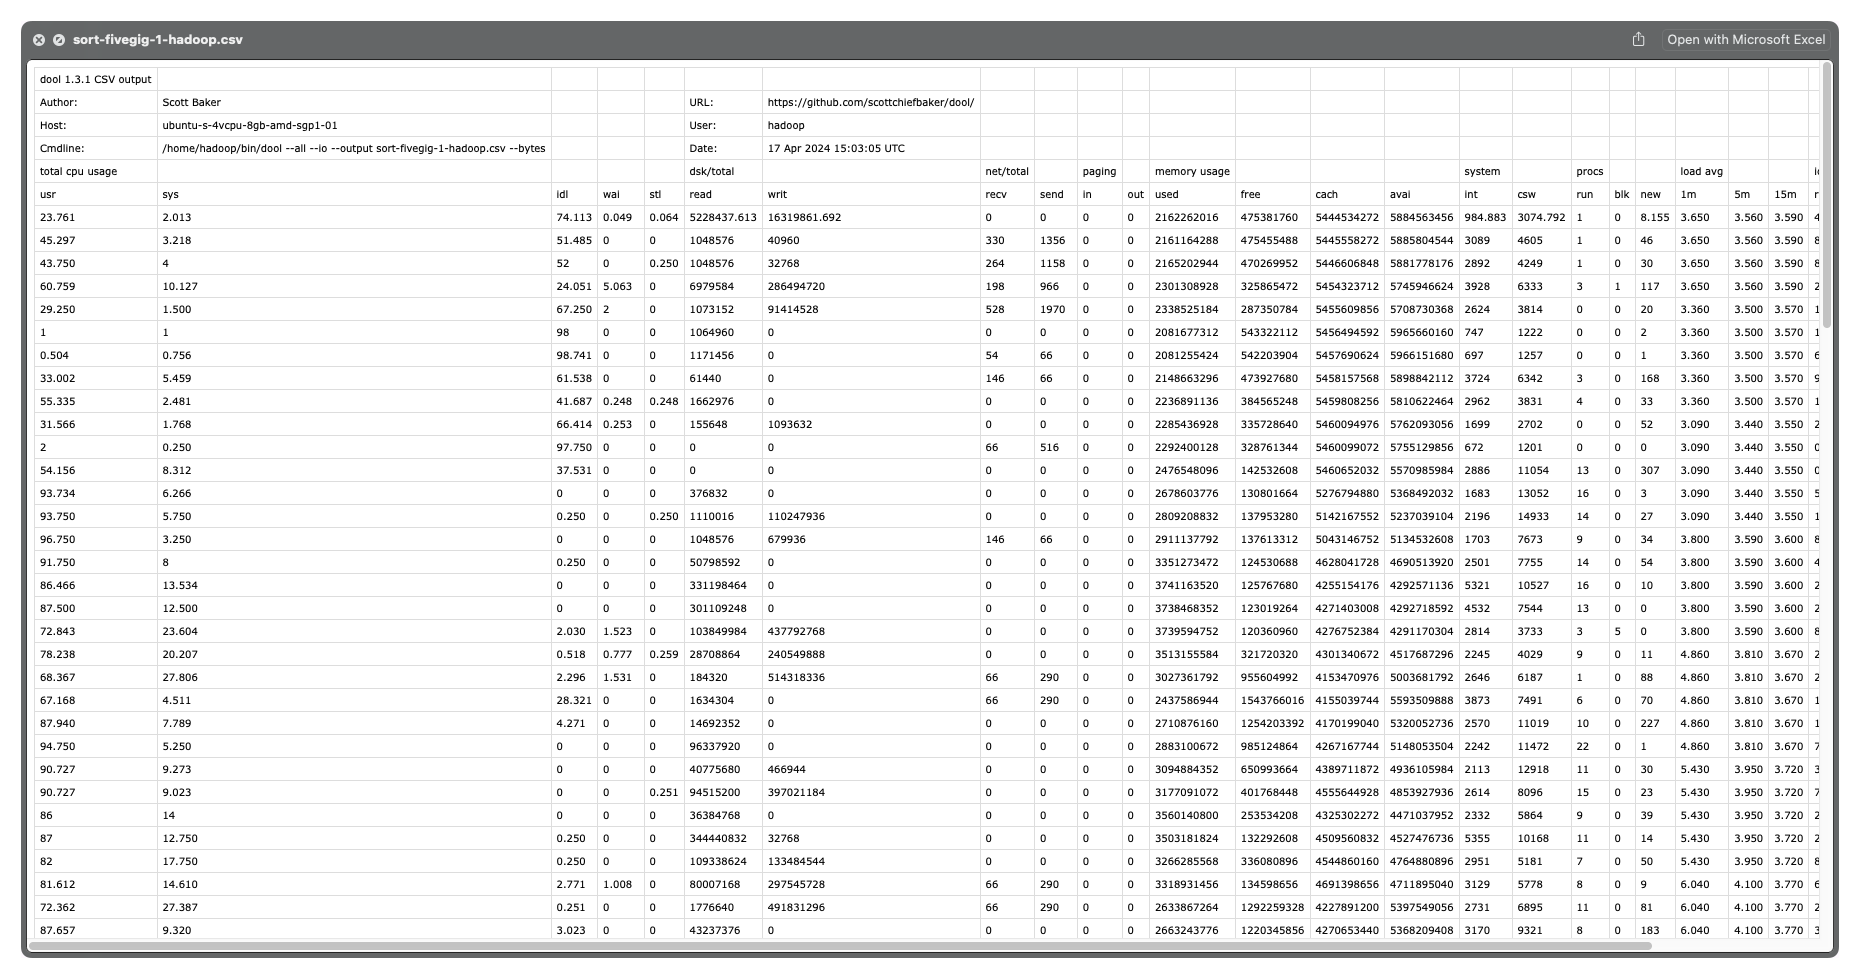
\includegraphics[width=\linewidth, height=0.5\linewidth]{figures/ch04/data-dool-dalam}
    \caption{Contoh Data Dool}
    \label{fig:data-dool-dalam}
\end{figure}
\end{landscape}

\newpage
\section {Analisis Kinerja}
\subsection{Persebaran Waktu Eksekusi pada Hadoop dan Spark}
Waktu eksekusi adalah waktu yang diperlukan dalam memproses data. Nilai parameter ini didapatkan dengan cara mencari selisih antara waktu awal dan waktu akhir saat Apache Hadoop dan Apache Spark dijalankan atau dihentikan untuk memproses input data dengan beban kerja masing-masing. Satuan pengukuran untuk parameter waktu eksekusi adalah detik atau \textit{second}. Setiap beban kerja dilakukan 5 perulangan untuk mendapatkan hasil yang lebih terukur. 

Gambar \ref{fig:lama-waktu-eksekusi-sort} dan \ref{fig:lama-waktu-eksekusi-wordcount} menyajikan \textit{scatter plot} yang membandingkan performa Hadoop dan Spark dalam dua tugas pemrosesan data yang berbeda, yaitu \textit{sort} dan \textit{word count}.  Sumbu x pada kedua gambar menunjukkan variasi ukuran input data, mulai dari 100 KB hingga 15 GB, sedangkan sumbu y menunjukkan waktu eksekusi dalam detik.

\begin{figure}[h]
    \centering
    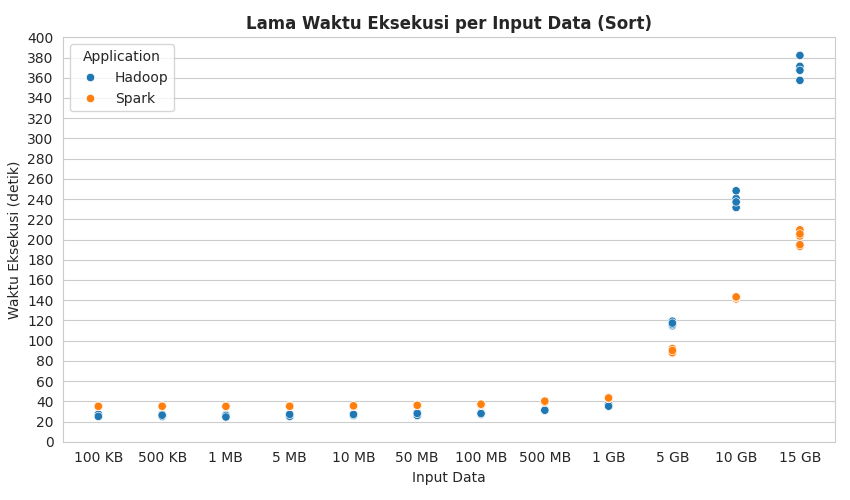
\includegraphics[width=1\textwidth]{figures/ch04/1-lama-waktu-eksekusi-sort.png}
    \caption{Persebaran Waktu Eksekusi \textit{Sort} (Hadoop, Spark)}
    \label{fig:lama-waktu-eksekusi-sort}
\end{figure}

Pada Gambar \ref{fig:lama-waktu-eksekusi-sort}, terlihat bahwa titik data waktu eksekusi Hadoop ketika input data 100 KB sampai 1 GB secara konsisten selalu berada di bawah titik data waktu eksekusi Spark, yang artinya Hadoop lebih cepat dibandingkan Spark. Hadoop berada pada rentang waktu 20-40 detik. Sedangkan, Spark berada pada rentang waktu yang lebih tinggi, yaitu sekitar 35-45 detik. 

Berbeda dengan input data 100 KB sampai 1 GB, Spark memiliki waktu eksekusi yang lebih cepat dibandingkan Hadoop ketika input data 5 GB. Spark berada pada rentang 80-100 detik, sedangkan Hadoop berada pada rentang 110-125 detik. Perbedaan performa ini semakin signifikan seiring bertambahnya ukuran data, yaitu pada 10 GB dan 15 GB. Gap perbedaan waktu eksekusi antara keduanya semakin jauh ketika input data ditambah dan pada beban kerja \textit{Sort}. 

\begin{figure}[h]
    \centering
    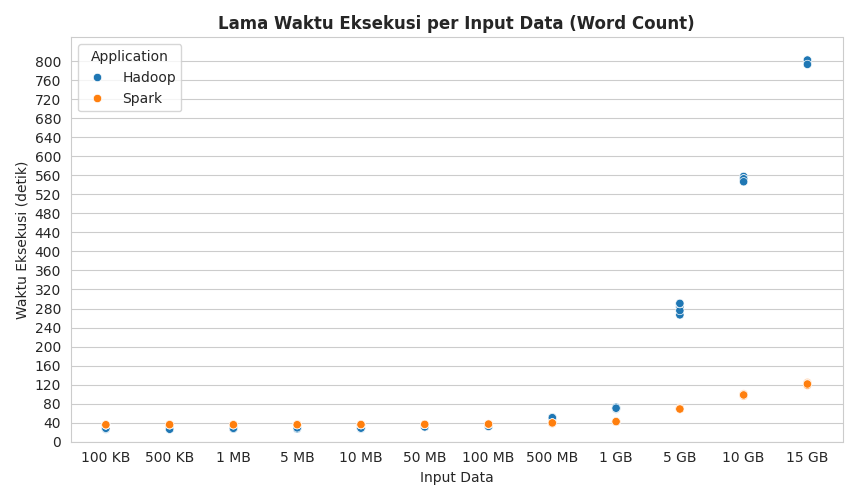
\includegraphics[width=1\textwidth]{figures/ch04/1-lama-waktu-eksekusi-wordcount.png}
    \caption{Persebaran Waktu Eksekusi \textit{Word Count} (Hadoop, Spark)}
    \label{fig:lama-waktu-eksekusi-wordcount}
\end{figure}

Pada Gambar \ref{fig:lama-waktu-eksekusi-wordcount}, Spark masih menunjukkan performa yang lebih baik daripada Hadoop pada ukuran input data 500 MB, 1 GB, 5 GB, 10 GB, dan 15 GB untuk beban kerja \textit{word count}. Namun, untuk ukuran input data 100 KB sampai 100 MB, Hadoop masih lebih baik. Lama waktu eksekusi Hadoop untuk input data 100 KB sampai 100 MB berada pada rentang 20-40 detik. Namun, perbedaannya tidak berbeda jauh dengan Spark karena titik data Hadoop-Spark saling menimpa (berdekatan).  

Hasil ini menunjukkan bahwa Spark lebih unggul dan konsisten daripada Hadoop dalam menangani tugas pemrosesan data yang lebih besar, dimana
\begin{enumerate}
	\item Untuk beban kerja \textit{sort}, Spark lebih unggul mulai dari input data 5 GB, 10 GB, dan 15 GB.
	\item Untuk beban kerja \textit{word count}, Spark lebih unggul mulai dari input data 500 MB, 1 GB, 5 GB, 10 GB, dan 15 GB. 
\end{enumerate}

% ----------------------------------------
\subsection {Persebaran \textit{Throughput} pada Hadoop dan Spark}

\textit{Throughput} adalah kecepatan pertukuran data per detik. Kegiatan pertukaran data tersebut terjadi pada \textit{node} yang dipakai dalam komputer komputasi, saat Hadoop maupun Spark memproses data. Oleh karena itu, semakin tinggi nilai \textit{throughput}, semakin sedikit waktu yang dibutuhkan untuk menyelesaikan komputasi. Satuan \textit{throughput} pada penelitian ini adalah MB/s (mega bita per detik). 

Gambar di bawah akan menyajikan scatter plot yang membandingkan \textit{throughput} Hadoop dan Spark dalam dua tugas pemrosesan data, yaitu \textit{sort} (Gambar \ref{fig:throughput-sort}) dan \textit{word count} (Gambar \ref{fig:throughput-wordcount}). Sumbu x pada kedua gambar menunjukkan variasi ukuran input data, sedangkan sumbu y menunjukkan \textit{throughput} dalam MB/s. 

\begin{figure}[h]
    \centering
    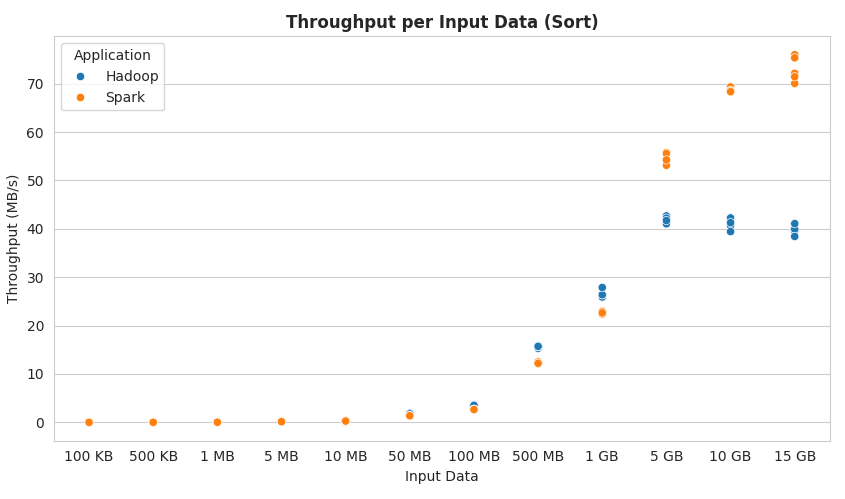
\includegraphics[width=1\textwidth]{figures/ch04/1-throughput-sort.png}
    \caption{\textit{Throughput Sort} (Hadoop, Spark)}
    \label{fig:throughput-sort}
\end{figure}

Pada tugas \textit{sort} (Gambar \ref{fig:throughput-sort}), Spark menunjukkan peningkatan \textit{throughput} yang signifikan seiring dengan bertambahnya ukuran data. Pada ukuran data terbesar (15 GB), Spark mencapai \textit{throughput} sekitar 70 MB/s. Sebaliknya, Hadoop menunjukkan peningkatan throughput yang lebih lambat dan hanya mencapai sekitar 40 MB/s pada ukuran data yang sama. Hal ini menunjukkan bahwa Spark mampu melakukan pertukaran data yang lebih besar daripada Hadoop.

\begin{figure}[h]
    \centering
    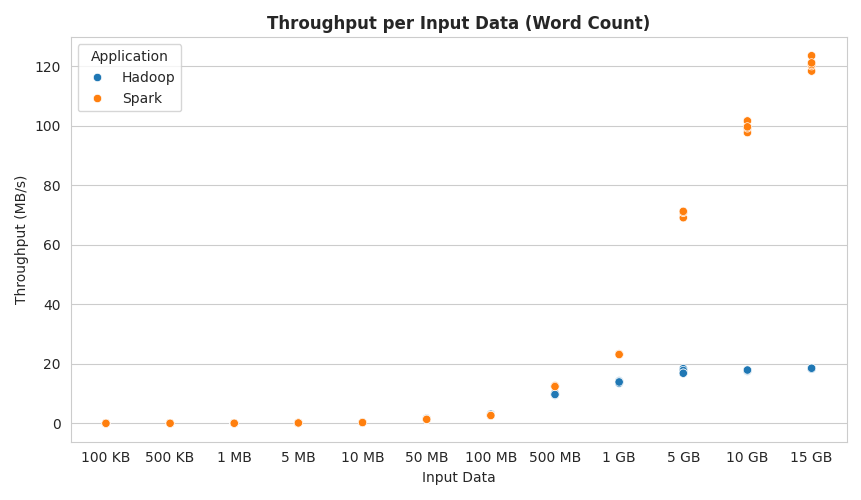
\includegraphics[width=1\textwidth]{figures/ch04/1-throughput-wordcount.png}
    \caption{\textit{Throughput Word Count} (Hadoop, Spark)}
    \label{fig:throughput-wordcount}
\end{figure}

Pada tugas \textit{word count} (Gambar \ref{fig:throughput-wordcount}), Spark mencapai throughput yang lebih tinggi daripada Hadoop. Perbedaan \textit{throughput} paling mencolok terlihat pada ukuran data terbesar (15 GB), di mana Spark mencapai \textit{throughput} lebih dari 120 MB/s, sedangkan Hadoop hanya mencapai sekitar 20 MB/s. Meskipun Spark menunjukkan peningkatan \textit{throughput} yang signifikan pada ukuran data besar (1 GB, 5 GB, 10 GB, dan 15 GB), pada data input yang lebih kecil, 100 KB sampai 100 MB, perbedaan \textit{throuhput} antara Hadoop dan Spark tidak berbeda jauh untuk \textit{word count}.

% ----------------------------------------

\subsection {Rata-rata Waktu Eksekusi pada Hadoop dan Spark}

Gambar \ref{fig:mean-dur-sort} dan \ref{fig:mean-dur-wordcount} menyajikan \textit{line plot} yang menggambarkan rata-rata waktu eksekusi Hadoop dan Spark untuk tugas \textit{sort} dan \textit{word count} dengan berbagai ukuran data. Sumbu x pada kedua gambar menunjukkan ukuran input data, sedangkan sumbu y menunjukkan rata-rata waktu eksekusi dalam detik. Garis vertikal pada kedua gambar menunjukkan titik di mana Spark mulai menunjukkan performa yang lebih cepat dibandingkan Hadoop.

\begin{figure}[h]
    \centering
    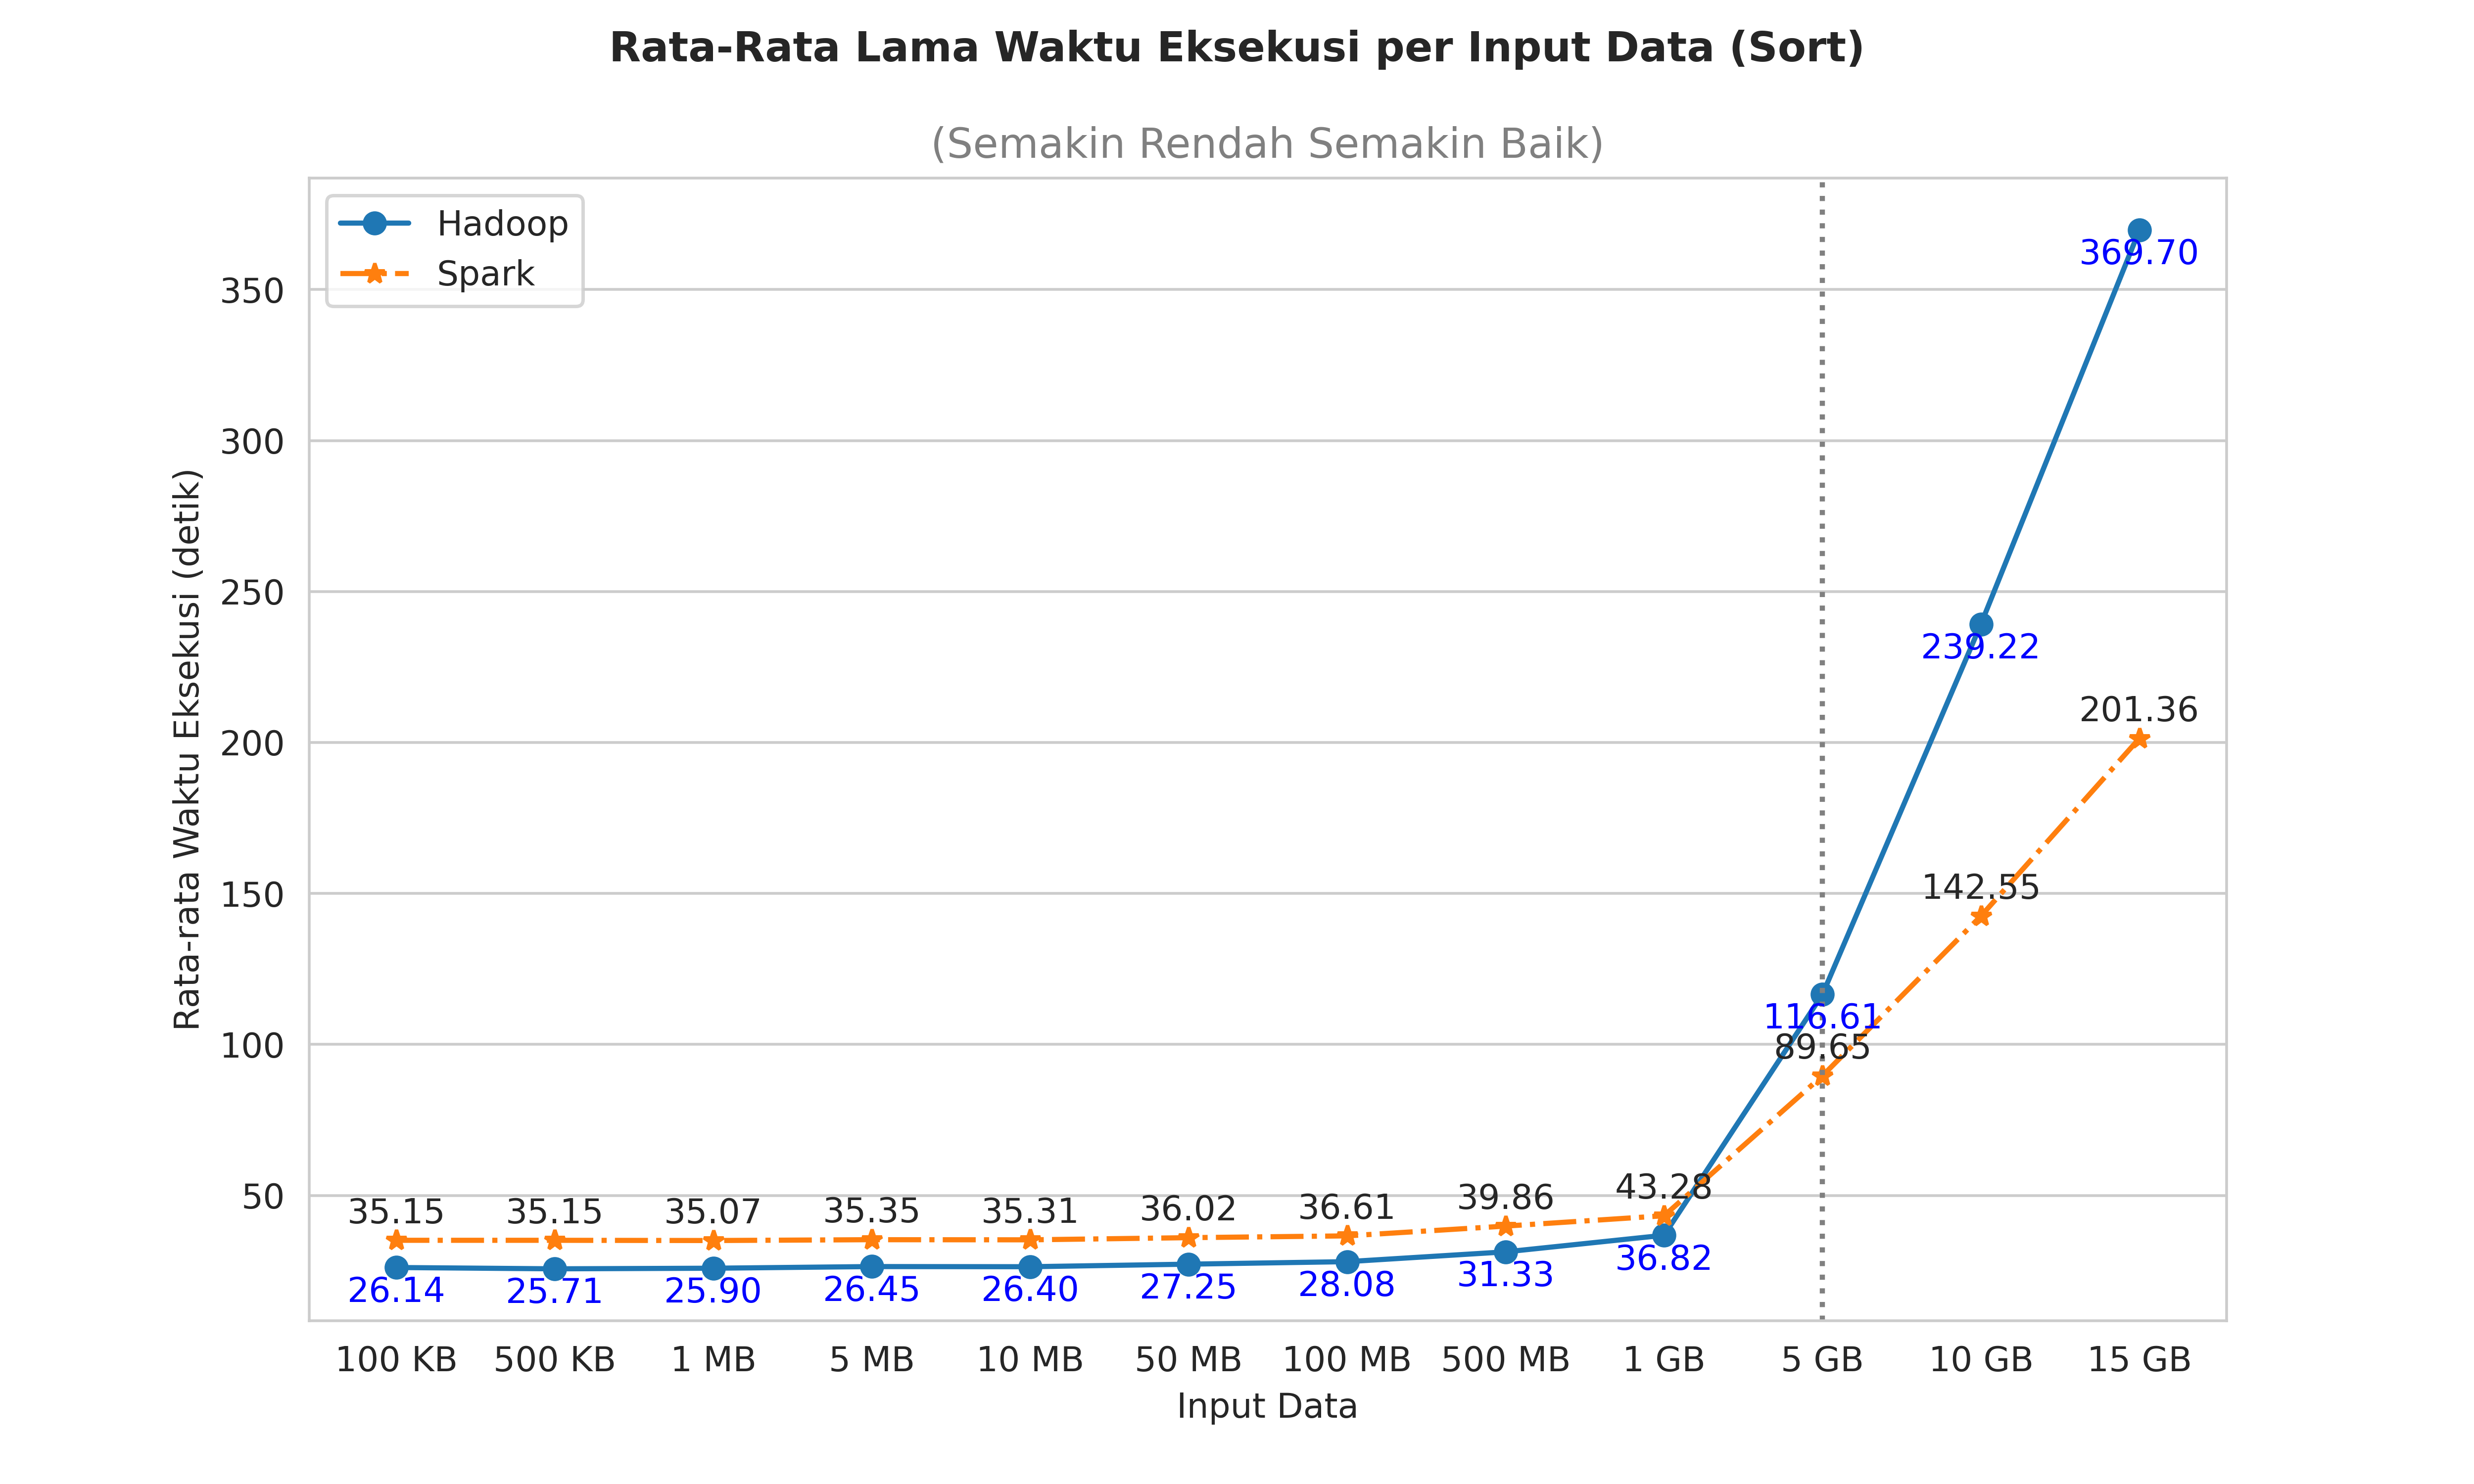
\includegraphics[width=1\textwidth]{figures/ch04/2-mean-lama-waktu-eksekusi-sort.png}
    \caption{Rata-rata Waktu Eksekusi \textit{(Sort)}}
    \label{fig:mean-dur-sort}
\end{figure}

Pada Gambar \ref{fig:mean-dur-sort}, terlihat bahwa Hadoop secara konsisten memiliki waktu eksekusi yang lebih rendah daripada Spark untuk ukuran input data 100 KB-1 GB pada tugas \textit{sort}. Perbedaan performa mulai terlihat pada input data 5 GB, dimana waktu eksekusi Spark mulai naik, namun tidak seperti Hadoop yang meningkat secara eksponensial.

\begin{figure}[h]
    \centering
    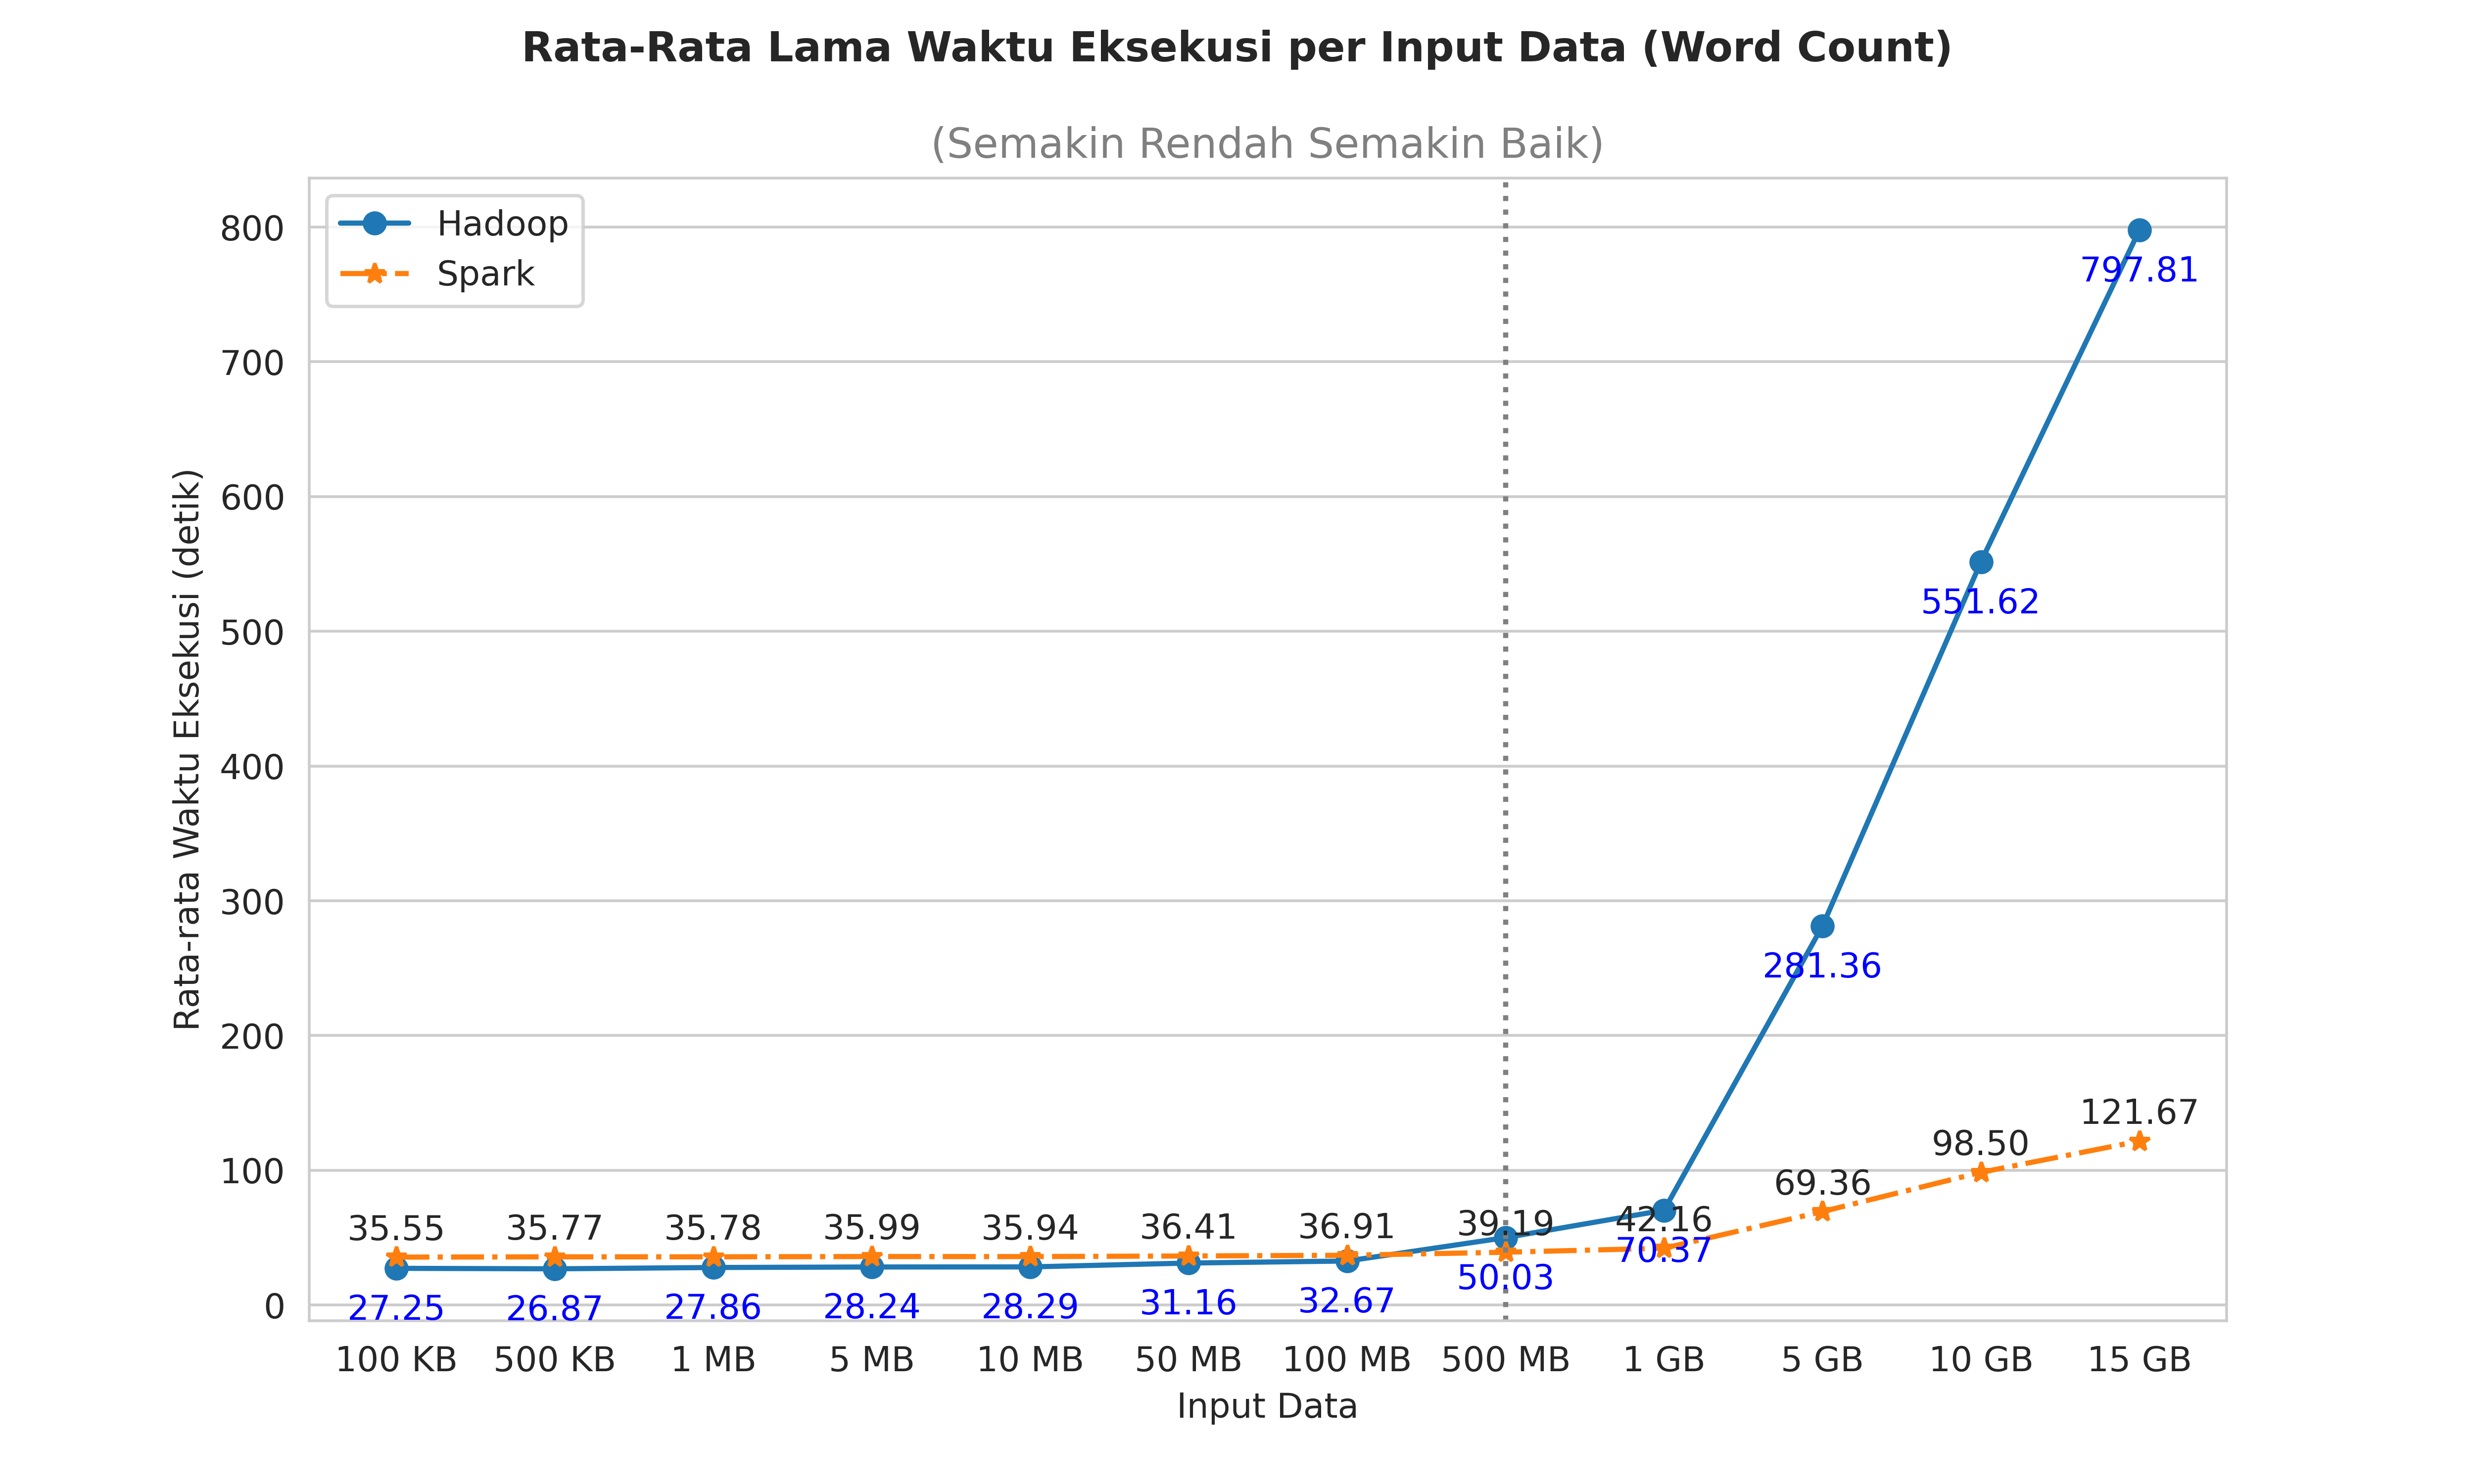
\includegraphics[width=1\textwidth]{figures/ch04/2-mean-lama-waktu-eksekusi-wordcount.png}
    \caption{Rata-rata Waktu Eksekusi \textit{(Word Count)}}
    \label{fig:mean-dur-wordcount}
\end{figure}

Pada Gambar \ref{fig:mean-dur-wordcount}, Spark juga menunjukkan performa yang lebih baik daripada Hadoop pada sebagian besar ukuran data pada tugas \textit{word count}, khususnya mulai dari input data 500 MB sampai 15 GB. Lama waktu eksekusi beban kerja pada Hadoop mulai mengalami kenaikan sejak input data 500 MB. Sedangkan, Spark baru mengalami kenaikan waktu eksekusi pada input data 5 GB.


% ----------------------------------------

\subsection {Rata-rata \textit{Throughput} pada Hadoop dan Spark}

Gambar \ref{fig:mean-throughput-sort} dan \ref{fig:mean-throughput-wordcount} menyajikan \textit{line plot} yang menggambarkan rata-rata throughput Hadoop dan Spark untuk tugas \textit{sort} dan \textit{word count} dengan berbagai ukuran data. Sumbu x pada kedua gambar menunjukkan ukuran input data, sedangkan sumbu y menunjukkan rata-rata \textit{throughput} dalam MB/s. Garis vertikal pada kedua gambar menunjukkan titik di mana Spark mulai menunjukkan throughput yang lebih tinggi dibandingkan Hadoop.

\begin{figure}[h]
    \centering
    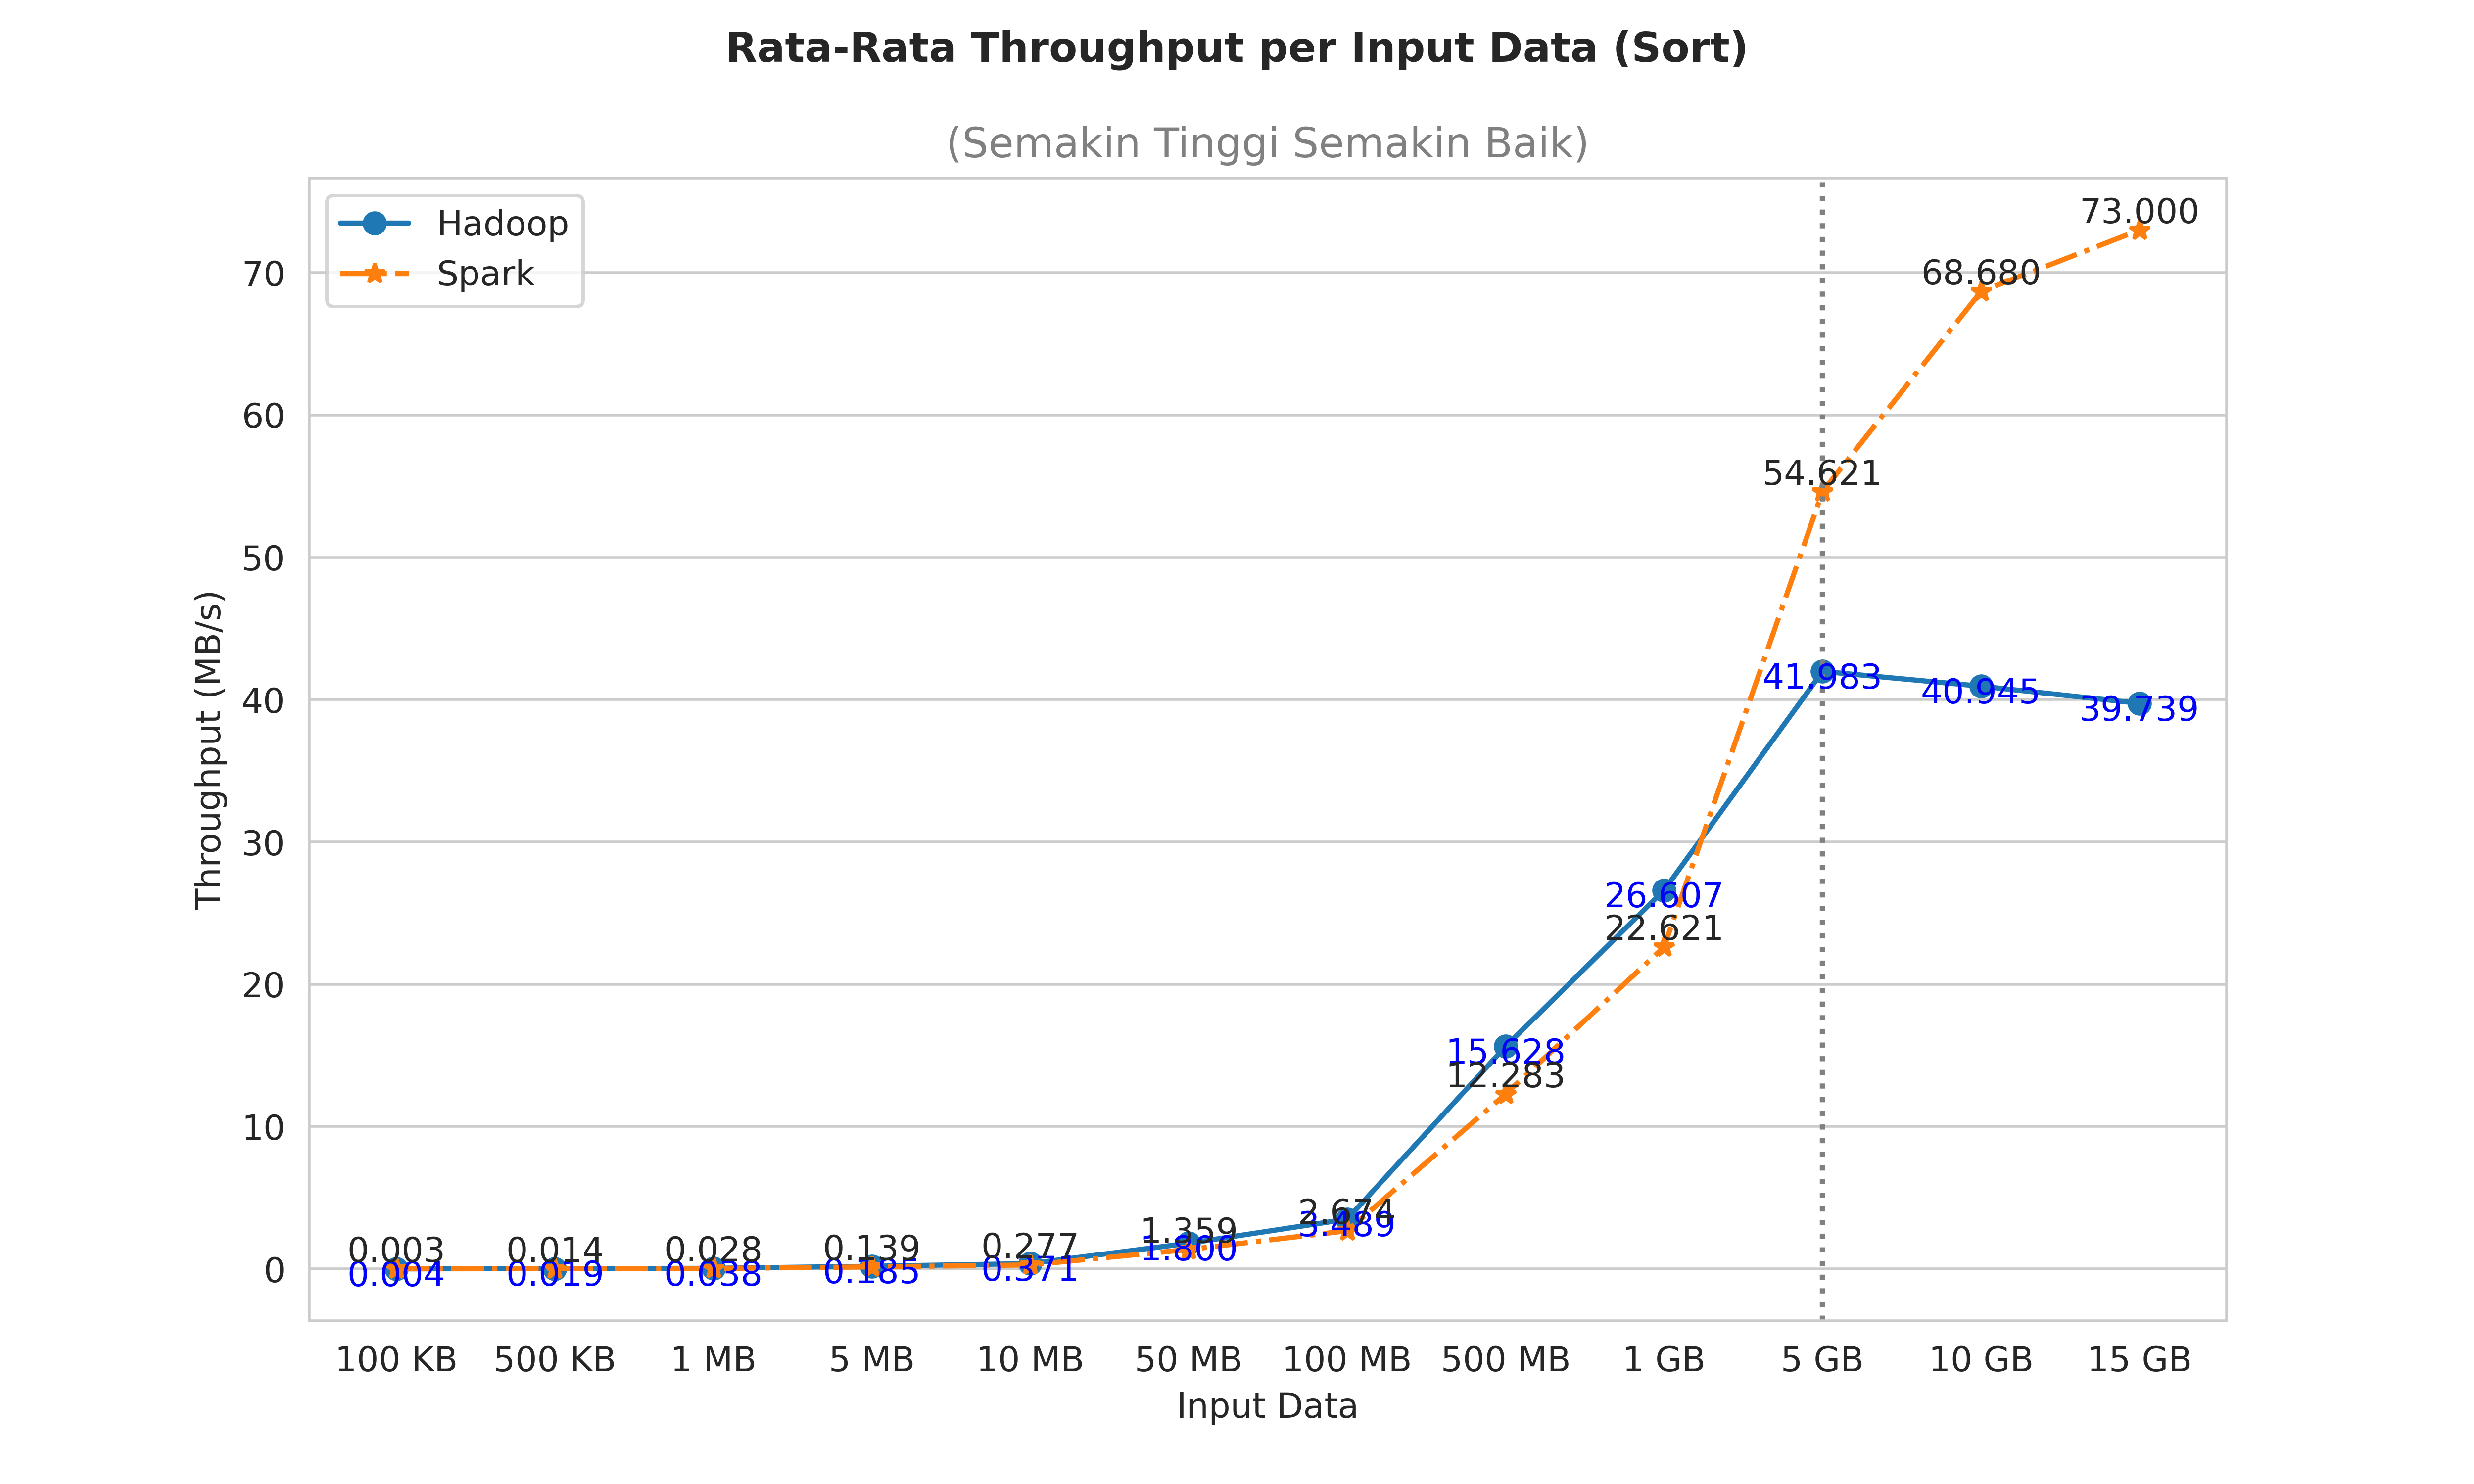
\includegraphics[width=0.85\textwidth]{figures/ch04/2-mean-throughput-sort.png}
    \caption{Rata-rata \textit{Throughput (Sort)}}
    \label{fig:mean-throughput-sort}
\end{figure}

Pada beban kerja \textit{sort}, Spark menunjukkan peningkatan \textit{throughput} yang signifikan seiring dengan meningkatnya ukuran data. Pada ukuran data kecil (di bawah 10 MB), \textit{throughput} Hadoop dan Spark relatif rendah dan sebanding. Setelah input data 10 MB, \textit{throughput} pada Hadoop meningkat dan sedikit menjauhi Spark. Namun, setelah input data 1 GB, Spark secara konsisten menunjukkan throughput yang lebih tinggi, mencapai 73.00 MB/s pada 15 GB dibandingkan dengan 41.98 MB/s untuk Hadoop. 

\begin{figure}[h]
    \centering
    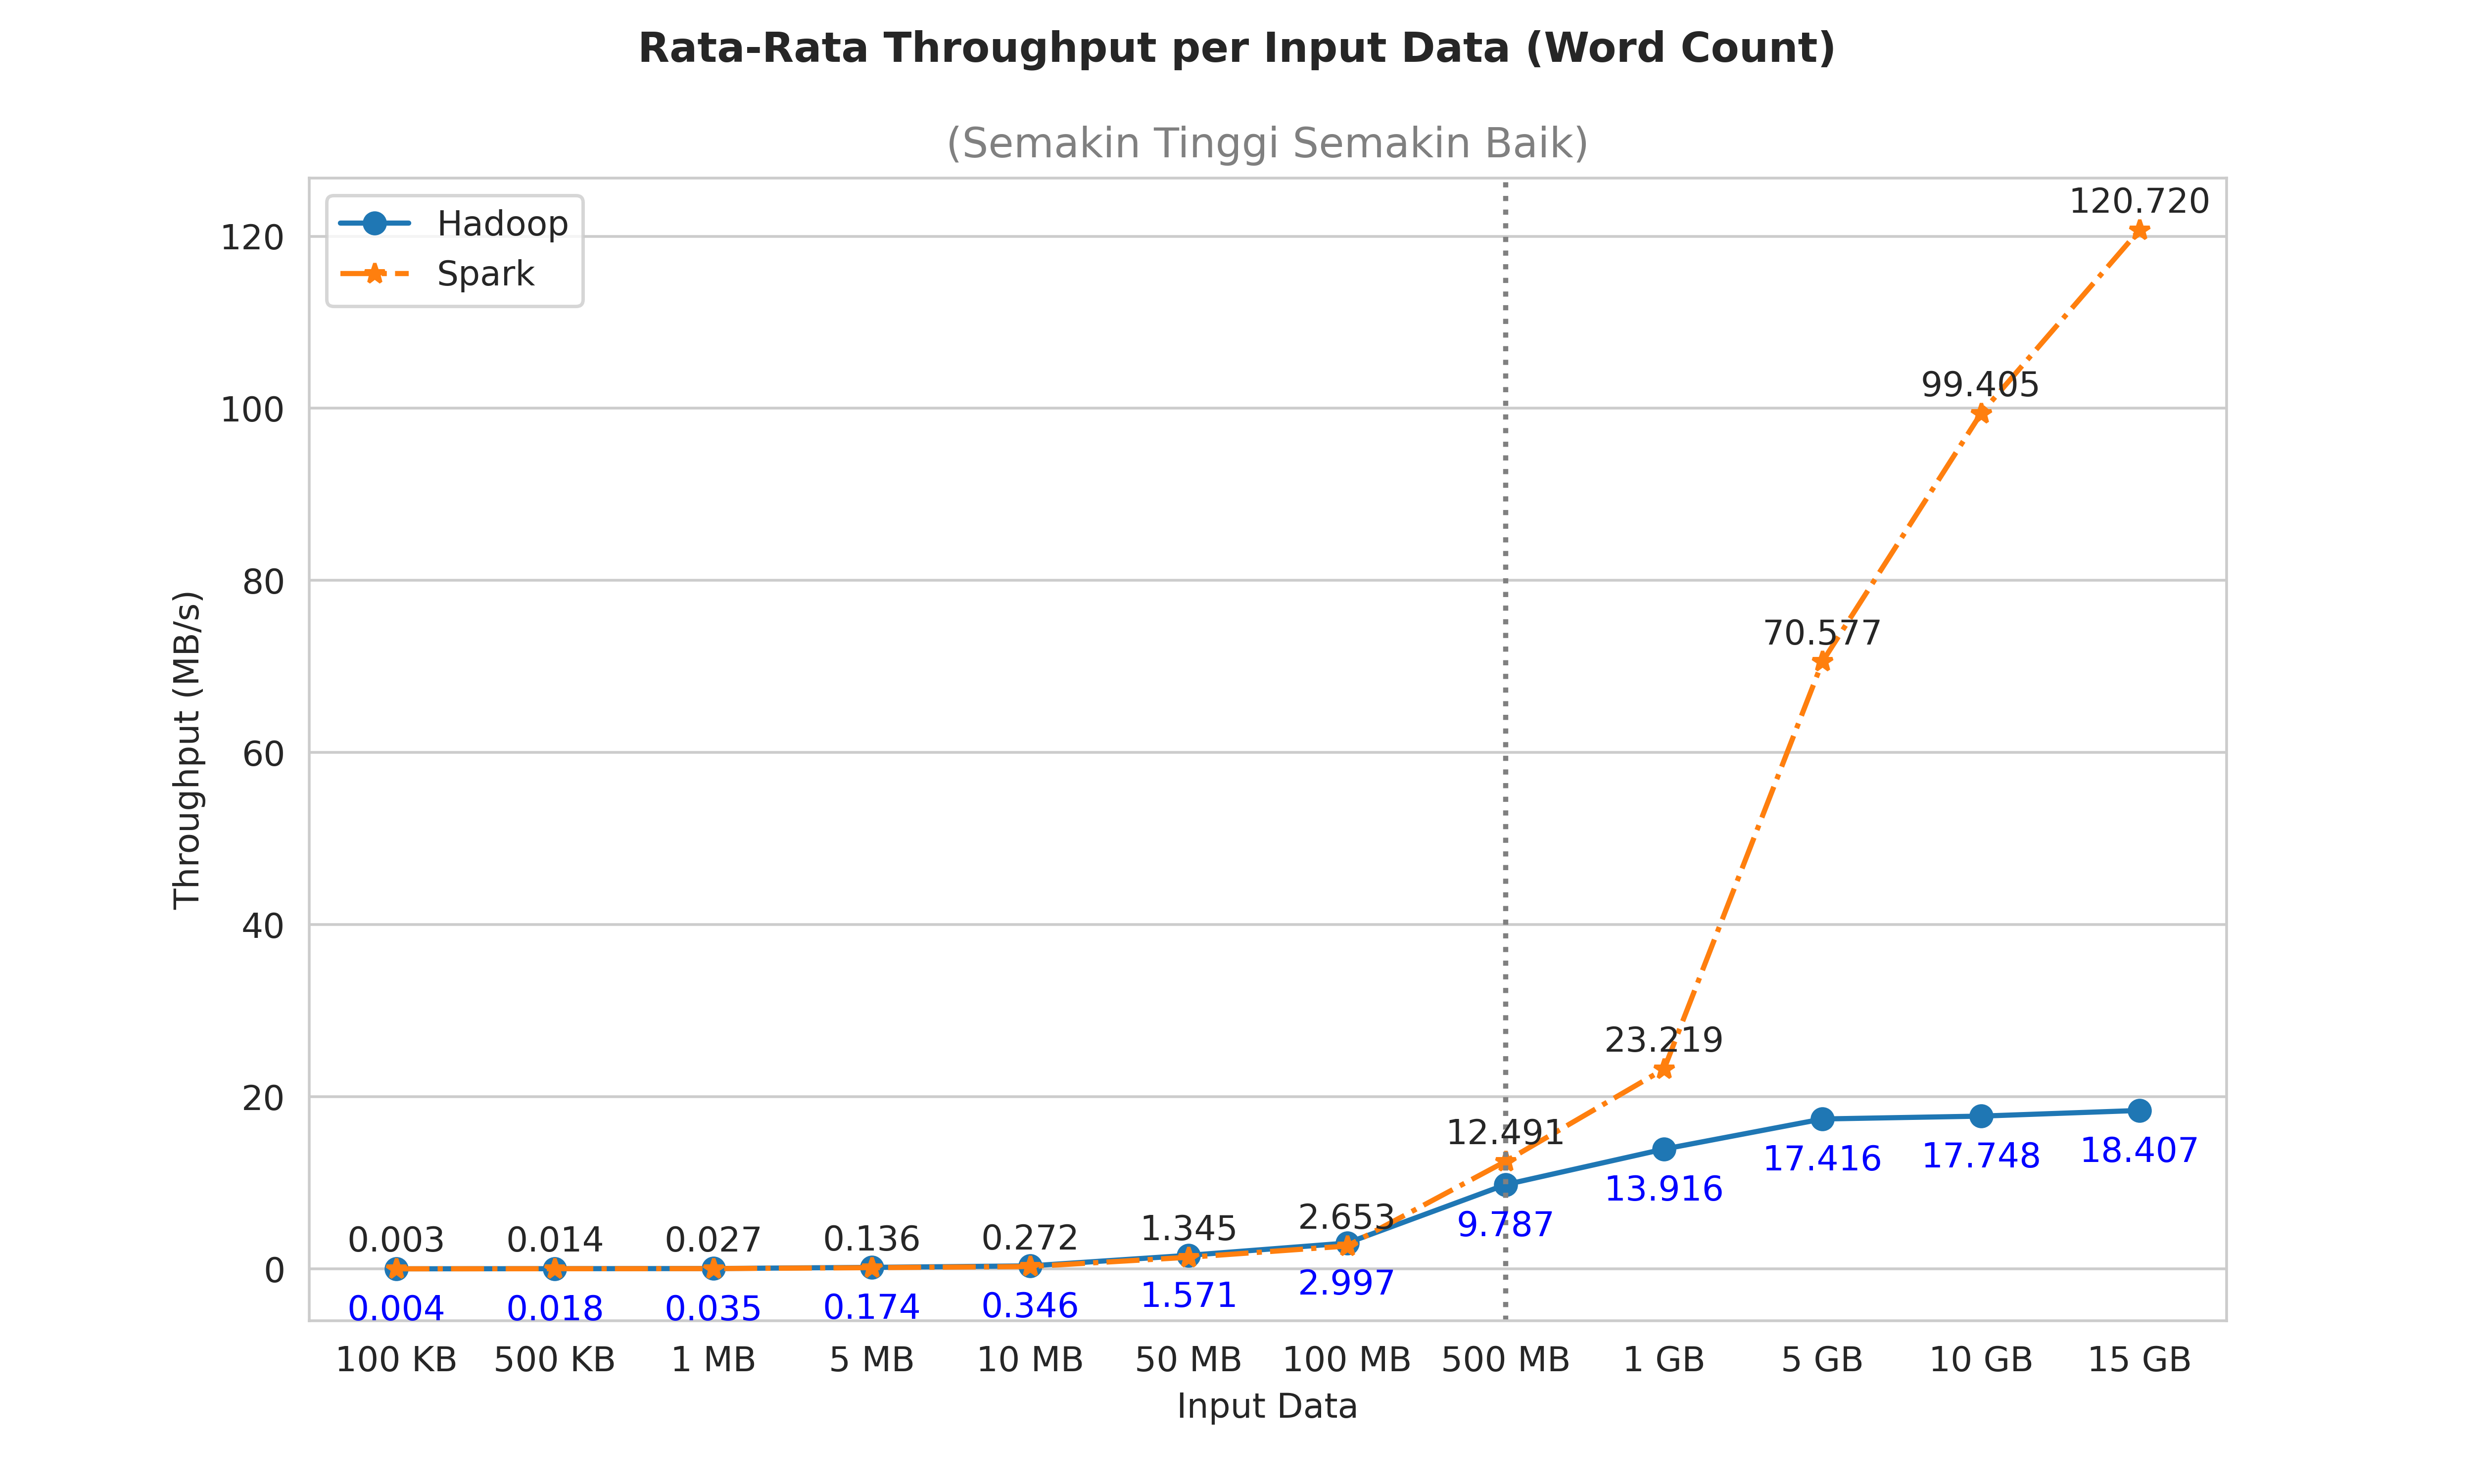
\includegraphics[width=0.85\textwidth]{figures/ch04/2-mean-throughput-wordcount.png}
    \caption{Rata-rata \textit{Throughput (Word Count)}}
    \label{fig:mean-throughput-wordcount}
\end{figure}

Pada beban kerja \textit{word count}, Spark juga mengungguli Hadoop dalam hal \textit{throughput} dengan perbedaan yang lebih besar daripada beban kerja \textit{sort}. Awalnya, \textit{throughput} Spark dan Hadoop sama dan saling berhimpit sejak input data 100 KB-100 MB. Spark mulai menunjukkan \textit{throughput} yang lebih tinggi pada ukuran data 500 MB.  Pada ukuran data 15 GB, Spark mencapai throughput 120 MB/s, sedangkan Hadoop hanya mencapai 18.407 MB/s.

%% --------------------------
%\newpage
%\subsection{Rate of Change}
%
%\begin{figure}[h]
%    \centering
%    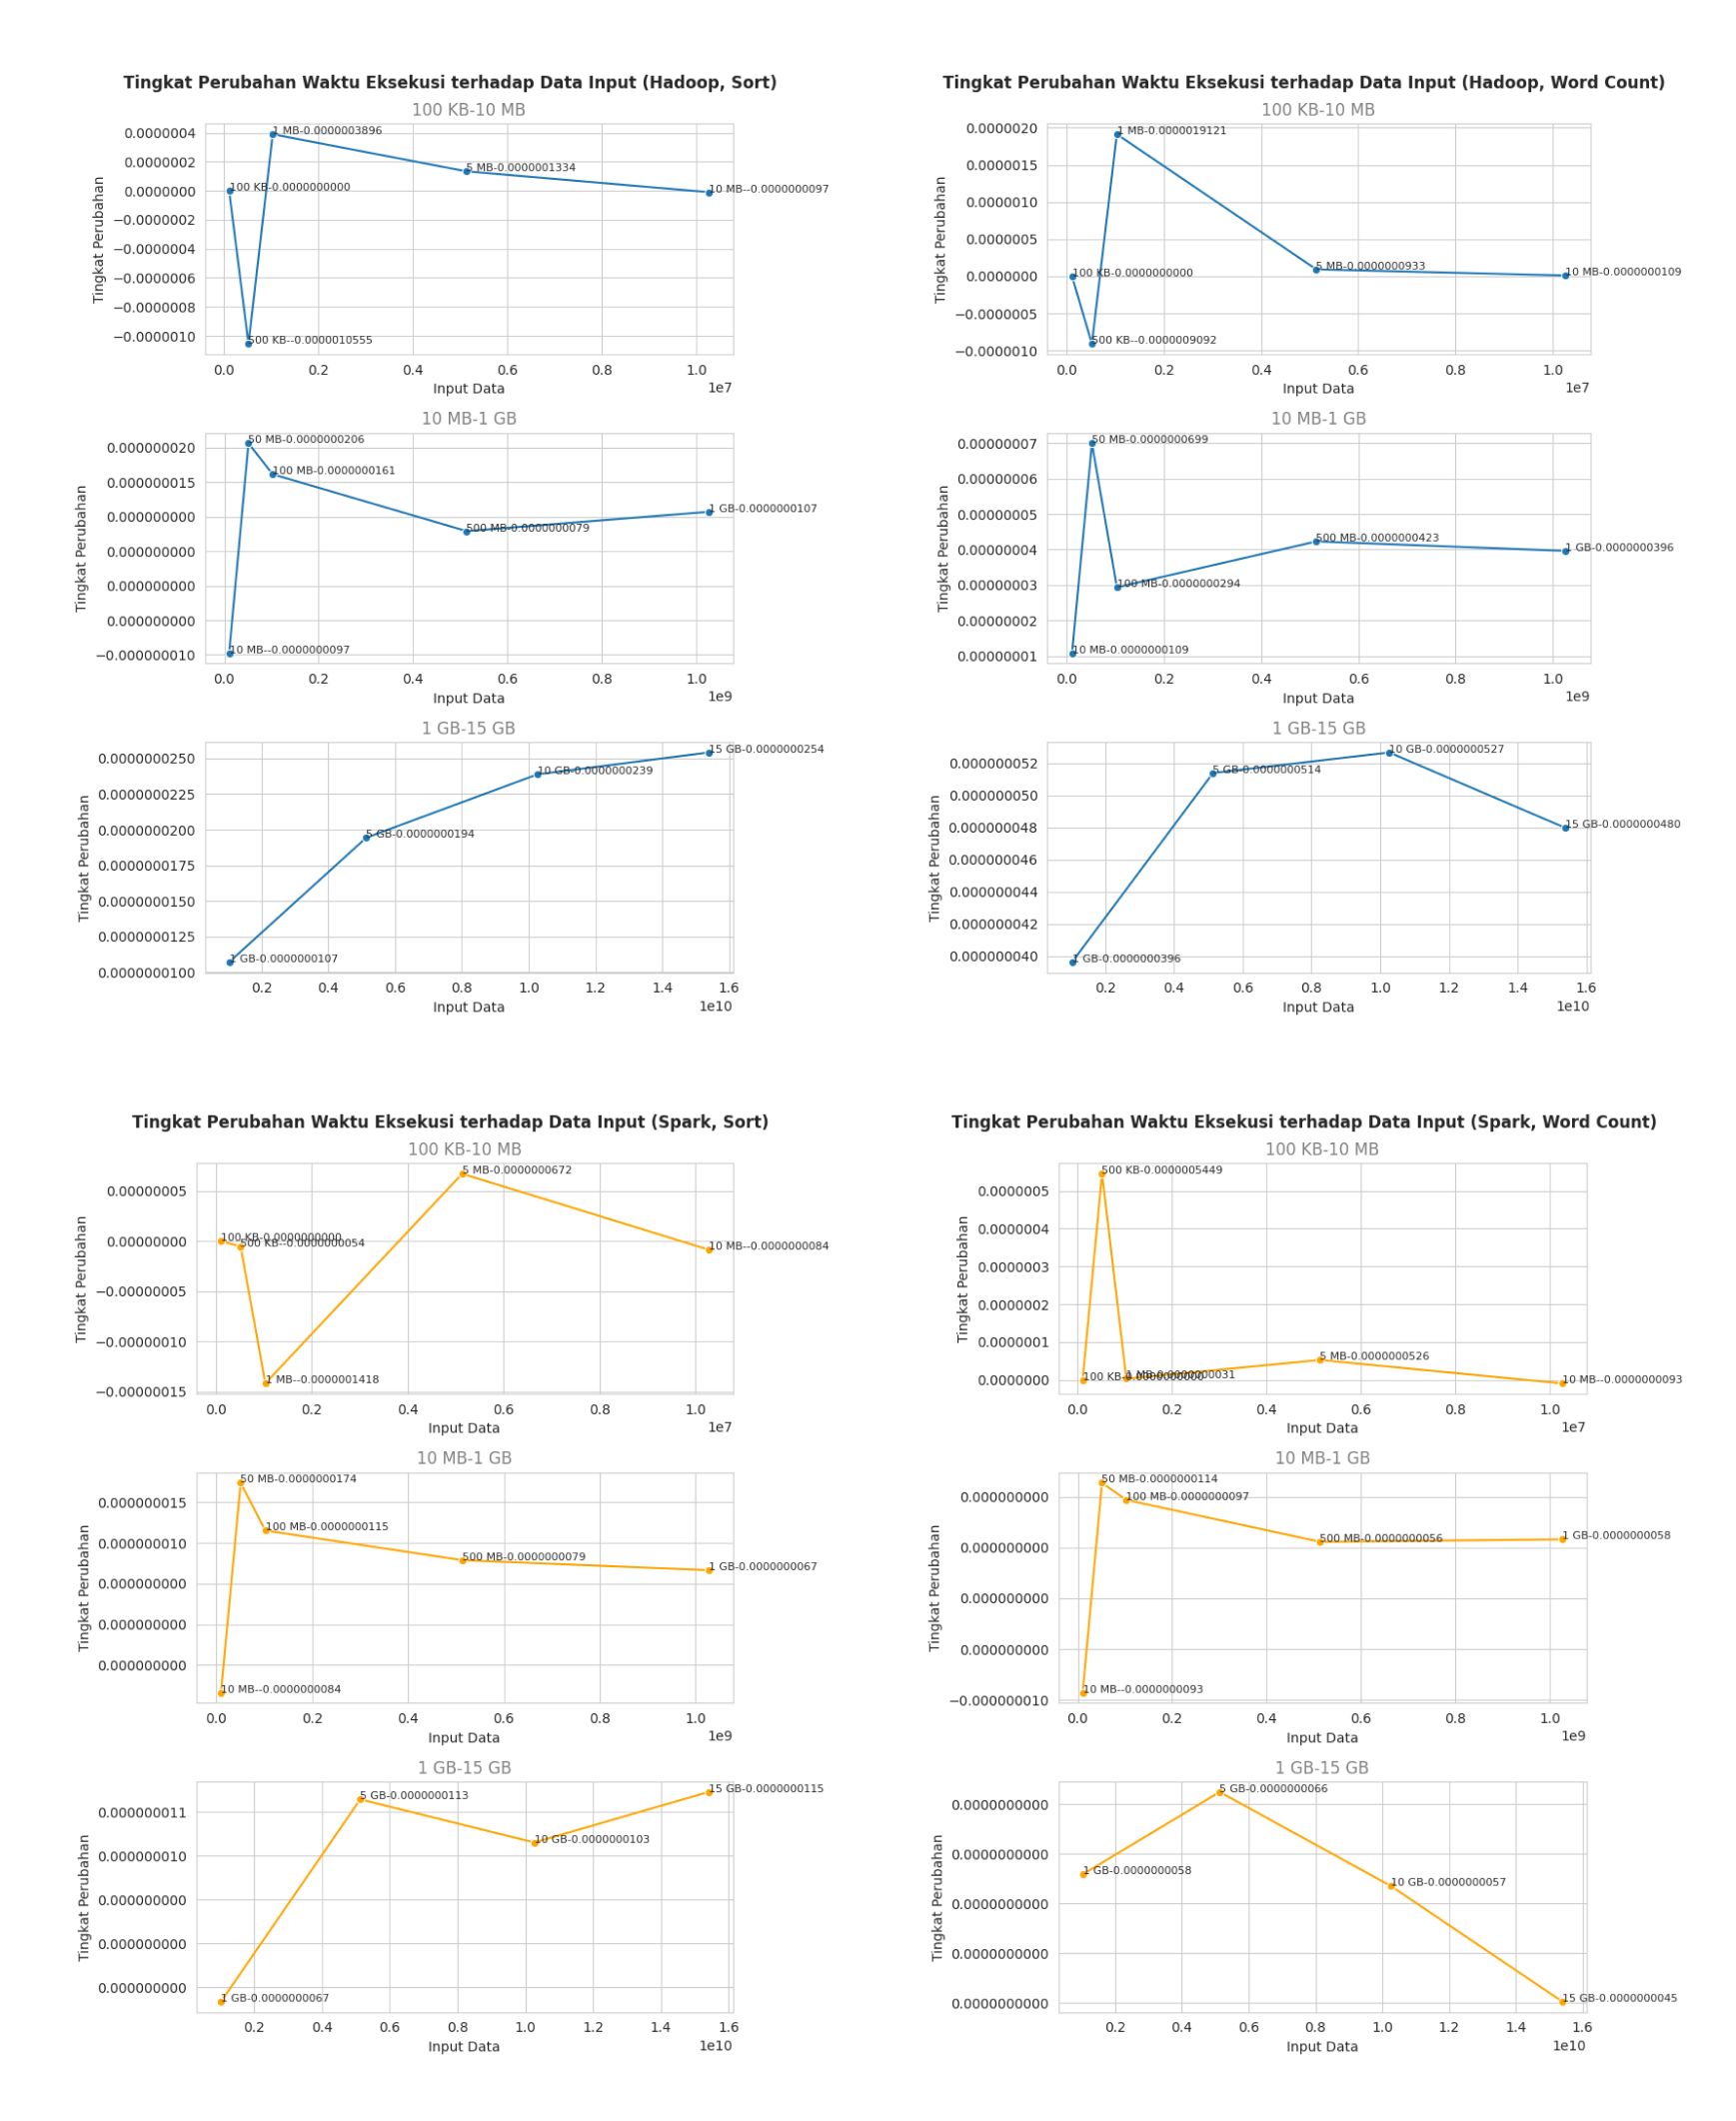
\includegraphics[width=1.1\textwidth]{figures/ch04/3-grup-dur.png}
%    \caption{dur}
%    \label{fig:3-grup-dur}
%\end{figure}
%
%\begin{figure}[h]
%    \centering
%    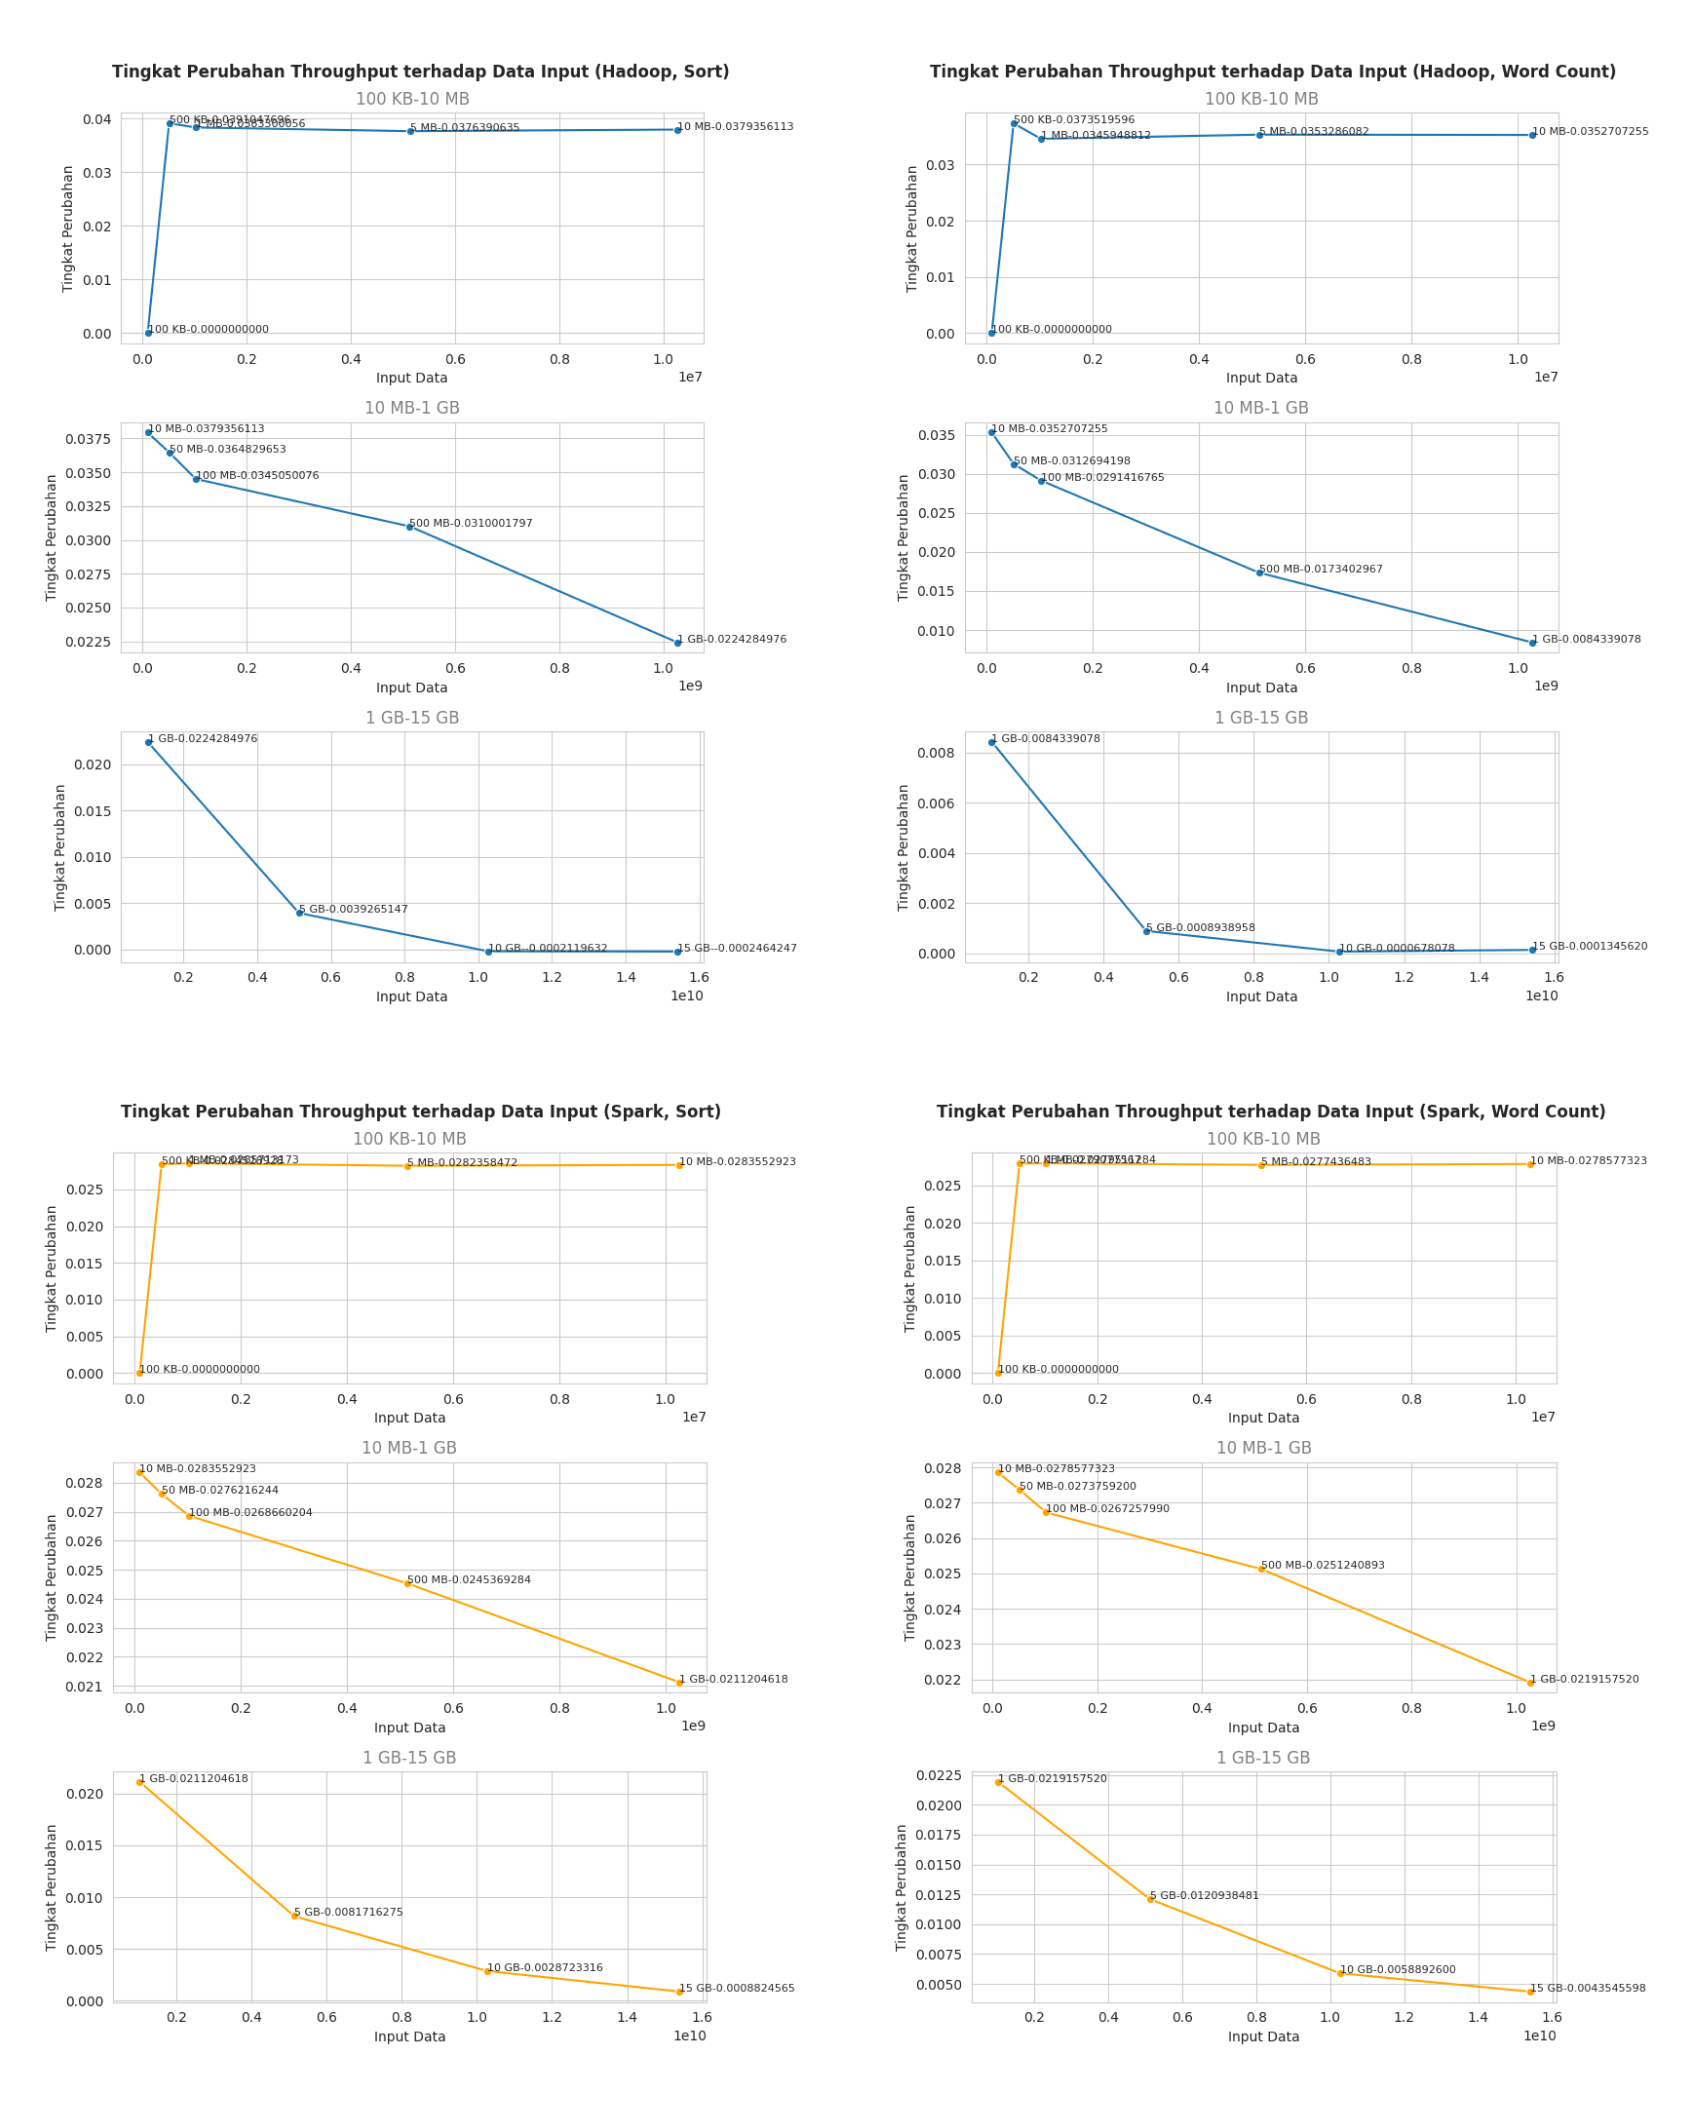
\includegraphics[width=1.1\textwidth]{figures/ch04/3-grup-th.png}
%    \caption{th}
%    \label{fig:3-grup-th}
%\end{figure}
%
%\begin{figure}[h]
%    \centering
%    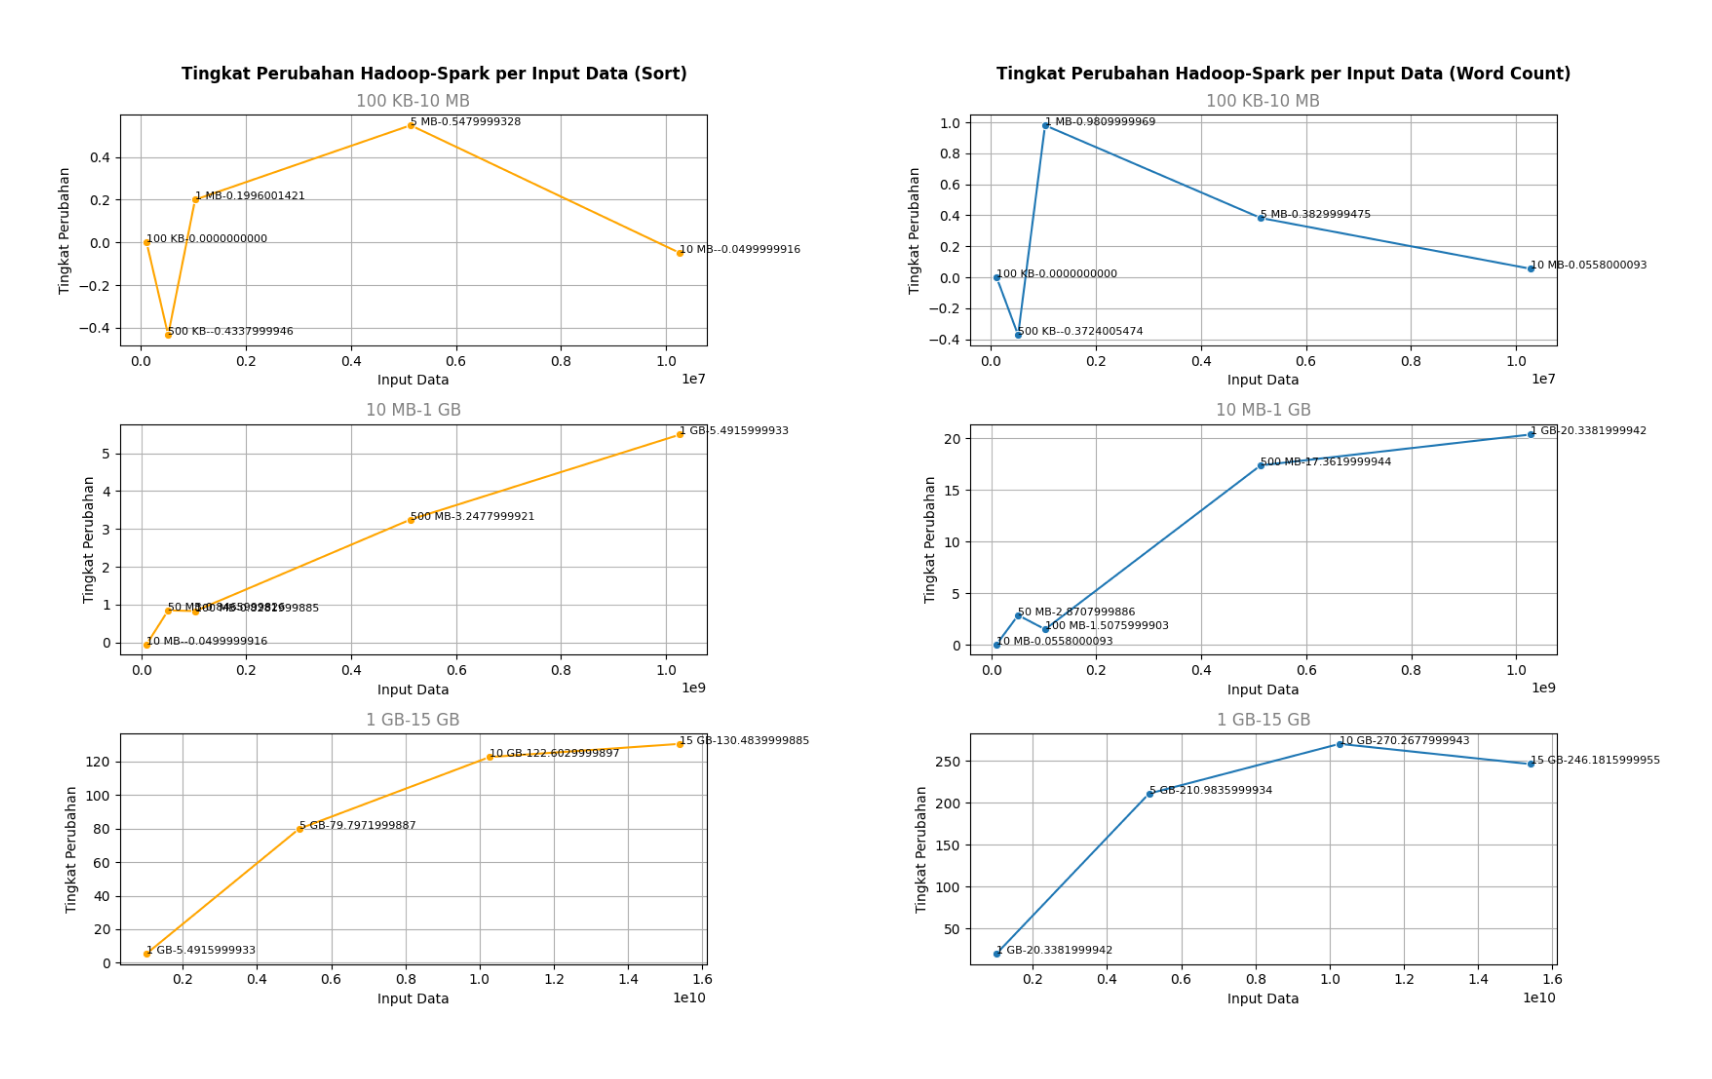
\includegraphics[width=1.1\textwidth]{figures/ch04/3-grup-hadoop-spark.png}
%    \caption{hadoop-spark}
%    \label{fig:3-grup-hadoop-spark}
%\end{figure}


% --------------------------------------

\newpage
\section{Analisis Penggunaan Sumber Daya}
\subsection{Penggunaan CPU}
Gambar \ref{fig:4-penggunaan-cpu-all-sort} dan \ref{fig:4-penggunaan-cpu-all-wordcount} menunjukkan pola penggunaan CPU oleh Hadoop dan Spark untuk beban kerja \textit{sort} dan \textit{word count} pada berbagai ukuran data. Sumbu x mewakili waktu dalam detik, sedangkan sumbu y mewakili persentase penggunaan CPU. Setiap grafik menunjukkan ukuran data yang berbeda, mulai dari 100 KB hingga 15 GB. Titik hitam menandakan titik perpotongan Hadoop dan Spark.

Pada beban kerja \textit{sort} (Gambar \ref{fig:4-penggunaan-cpu-all-sort}), perbedaan pola penggunaan CPU antara Hadoop dan Spark semakin terlihat pada ukuran data yang lebih besar. Jika dilihat pada input data 100 KB-1 GB, penggunaan CPU pada masing-masing Hadoop dan Spark tidak berbeda jauh. Selanjutnya, pada input data 5 GB, 10 GB, dan 15 GB, penggunaan CPU Hadoop sangat fluktuatif berkisar pada 60\%-95\% pada dua per tiga bagian waktu awal eksekusi, dan pada satu per tiga waktu eksekusi mengalami penurunan yang berkisar pada 20\%-80\%. Berbeda dengan Hadoop, Spark memiliki penggunaan CPU yang lebih stabil (terkadang pada 60\%-80\%, dan terkadang pada 80\%-100\%).

Pada beban kerja \textit{word count} (Gambar \ref{fig:4-penggunaan-cpu-all-wordcount}), Hadoop menunjukkan penggunaan CPU yang lebih fluktuatif (naik turun) dan tinggi secara keseluruhan dibandingkan dengan Spark. Penggunaan CPU pada 10 detik pertama pada Hadoop berkisar pada 10\%-60\% . Setelah itu, penggunaan CPU-nya naik sampai ke 100\% dan naik turun. Jika dilihat dari input data yang lebih besar (15 GB), Hadoop memiliki pola CPU yang hampir sama pada setiap data input, yaitu 10 detik pertama berada pada 10\%-60\%, setengah pertama naik turun pada penggunaan CPU 60\%-100\%, dan setengah terakhir menurunkan penggunaan CPU pada 50\%-90\%. Selanjutnya, Spark juga memiliki pola tersendiri. Penggunaan CPU Spark pada detik pertama sampai detik ke 15 fluktuatif pada 20\%-50\%, hingga pada detik 16 sampai detik ke 35 turun ke 0\%, dan baru naik lagi pada detik ke 35. Hal yang menarik juga adalah penggunaan CPU Spark tidak menyentuh 100\%, tetapi memiliki waktu eksekusi beban kerja yang lebih cepat pada \textit{word count}. 

Pada kedua tugas, terlihat bahwa beban kerja \textit{word count} cenderung menunjukkan pola penggunaan CPU yang lebih tinggi dan konsisten dibandingkan dengan beban kerja \textit{sort}. Pada beban kerja \textit{word count}, umumnya penggunaan CPU Hadoop lebih tinggi dan merata di sepanjang waktu eksekusi jika dibandingkan dengan Spark. Di sisi lain, beban kerja \textit{sort} menunjukkan penggunaan CPU yang cenderung lebih fluktuatif, dengan periode lonjakan dan penurunan yang signifikan, baik pada Hadoop maupun Spark. 

\begin{landscape}
\begin{figure}[h]
    \centering
    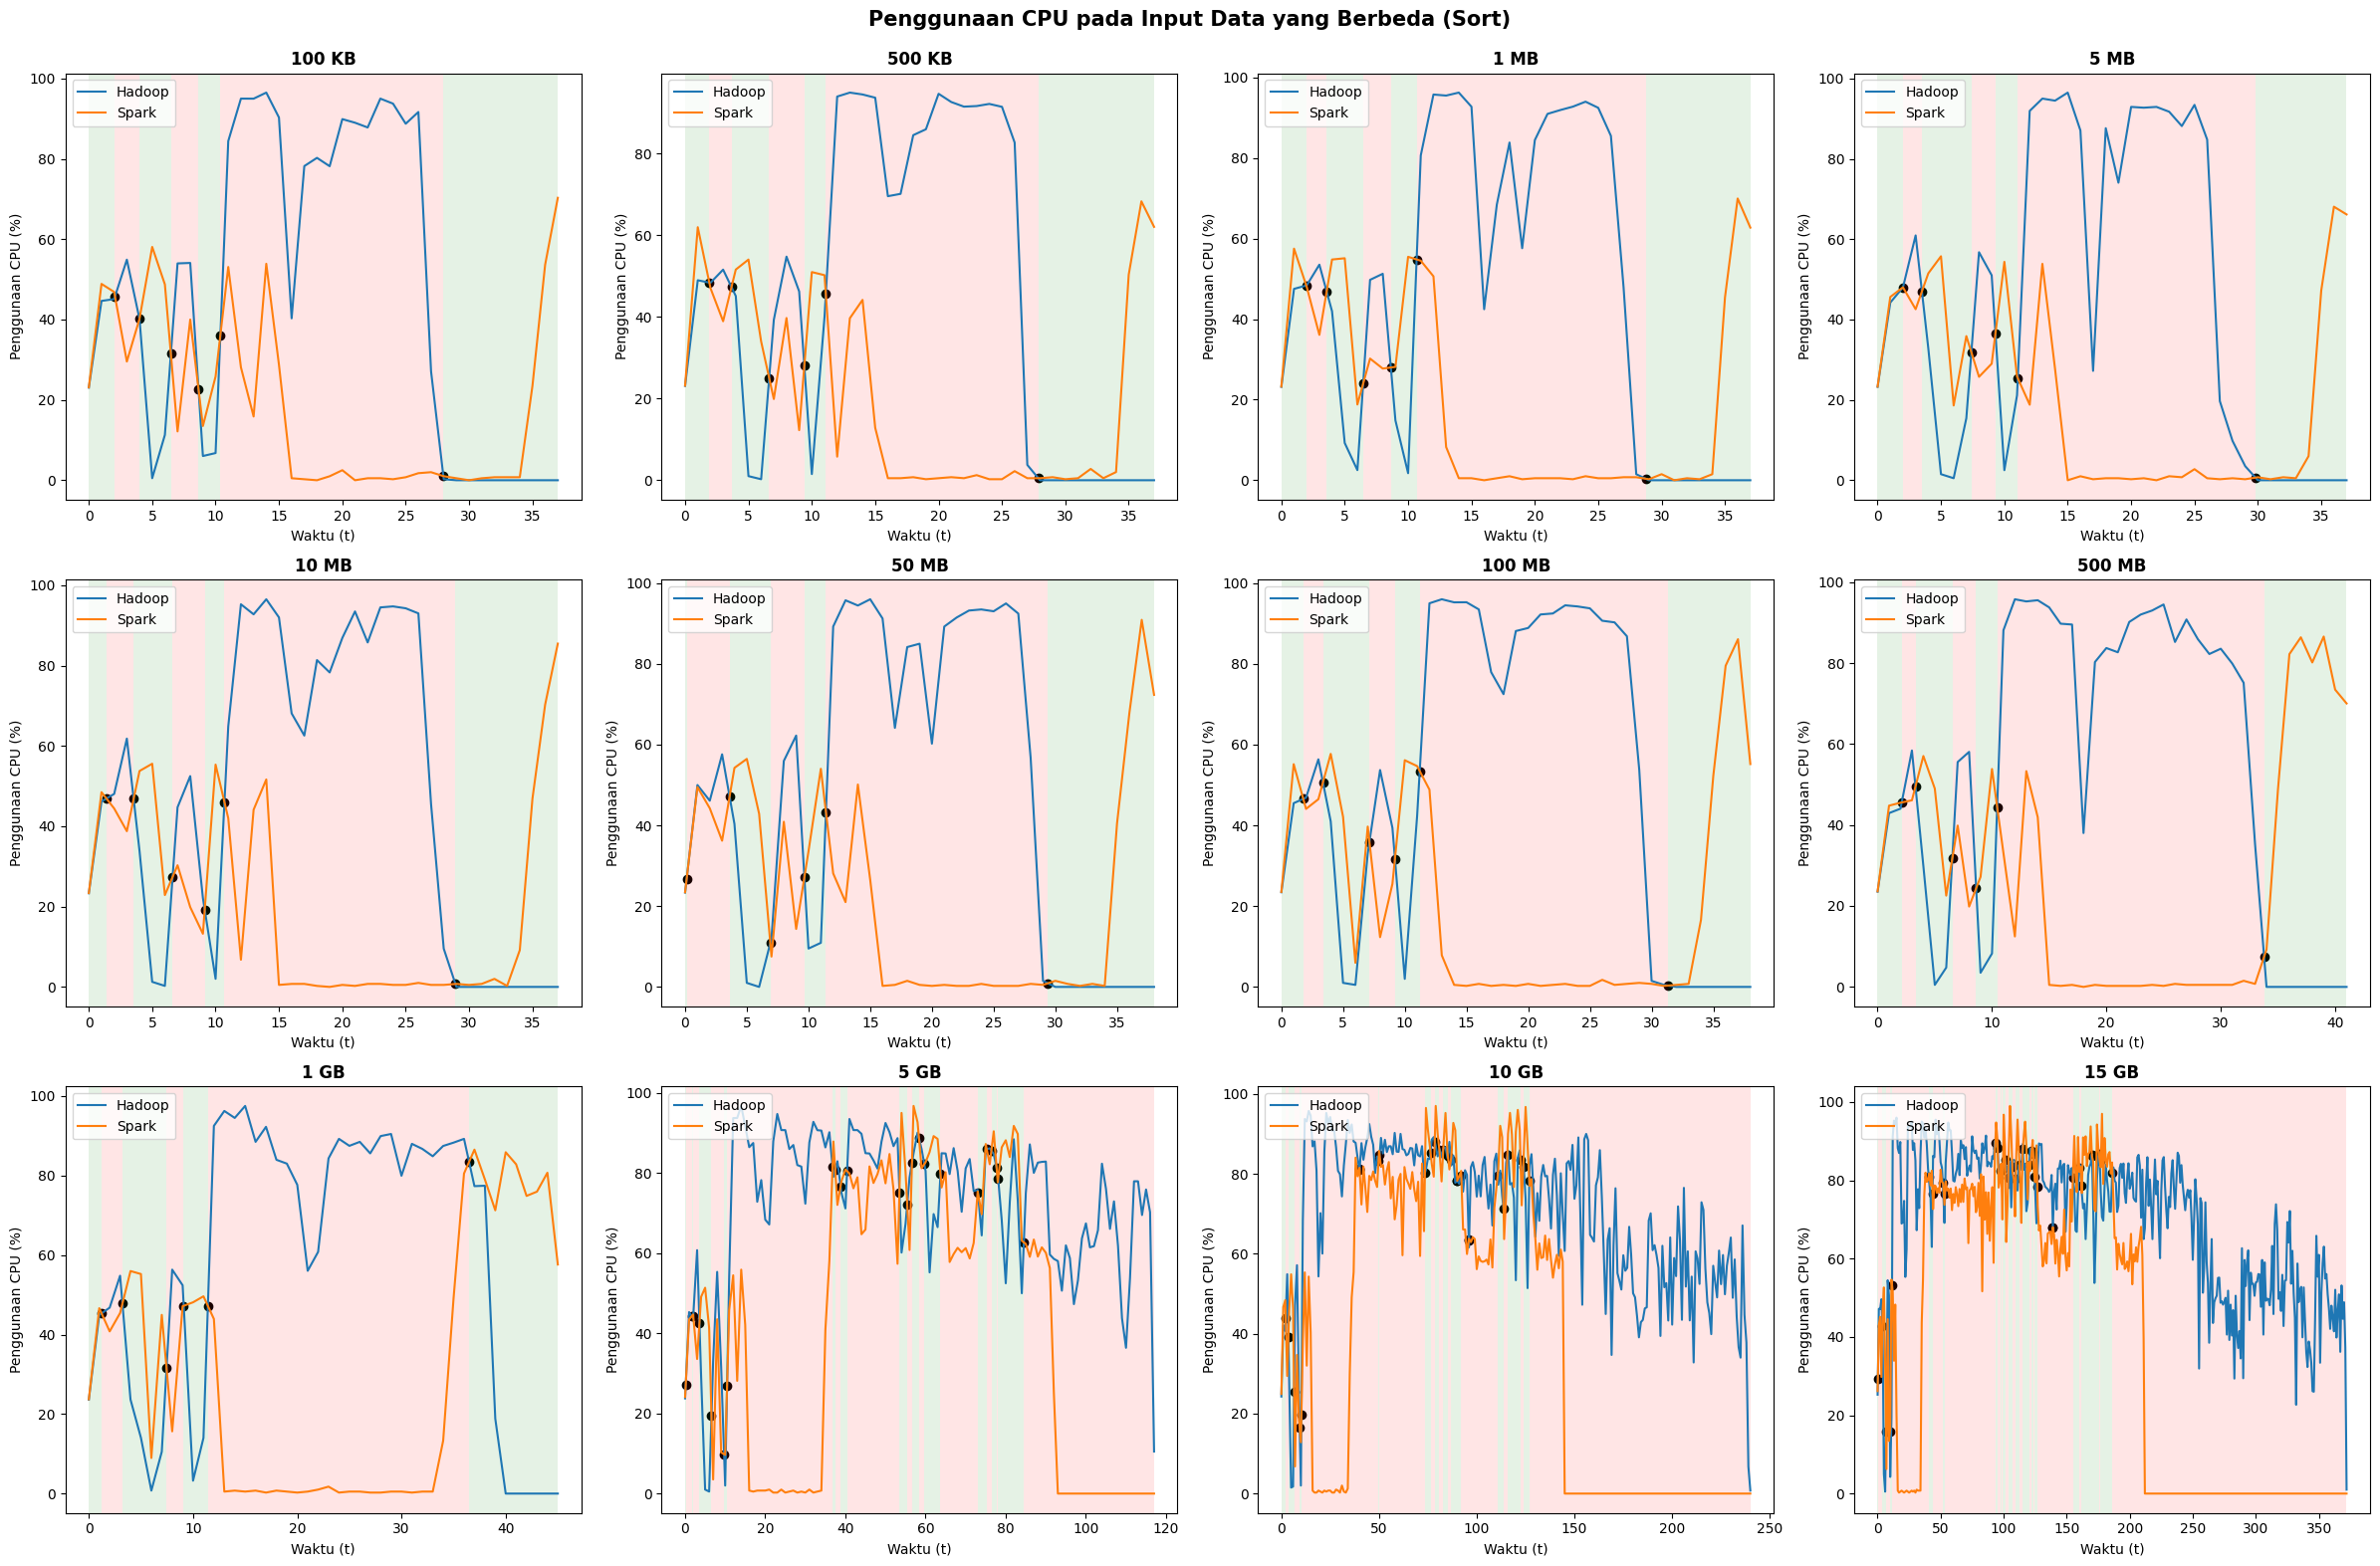
\includegraphics[height=0.6\linewidth]{figures/ch04/4-penggunaan-cpu-all-sort.png}
    \caption{Penggunaan CPU (\textit{Sort})}
    \label{fig:4-penggunaan-cpu-all-sort}
\end{figure}
\end{landscape}

\begin{landscape}
\begin{figure}[h]
    \centering
    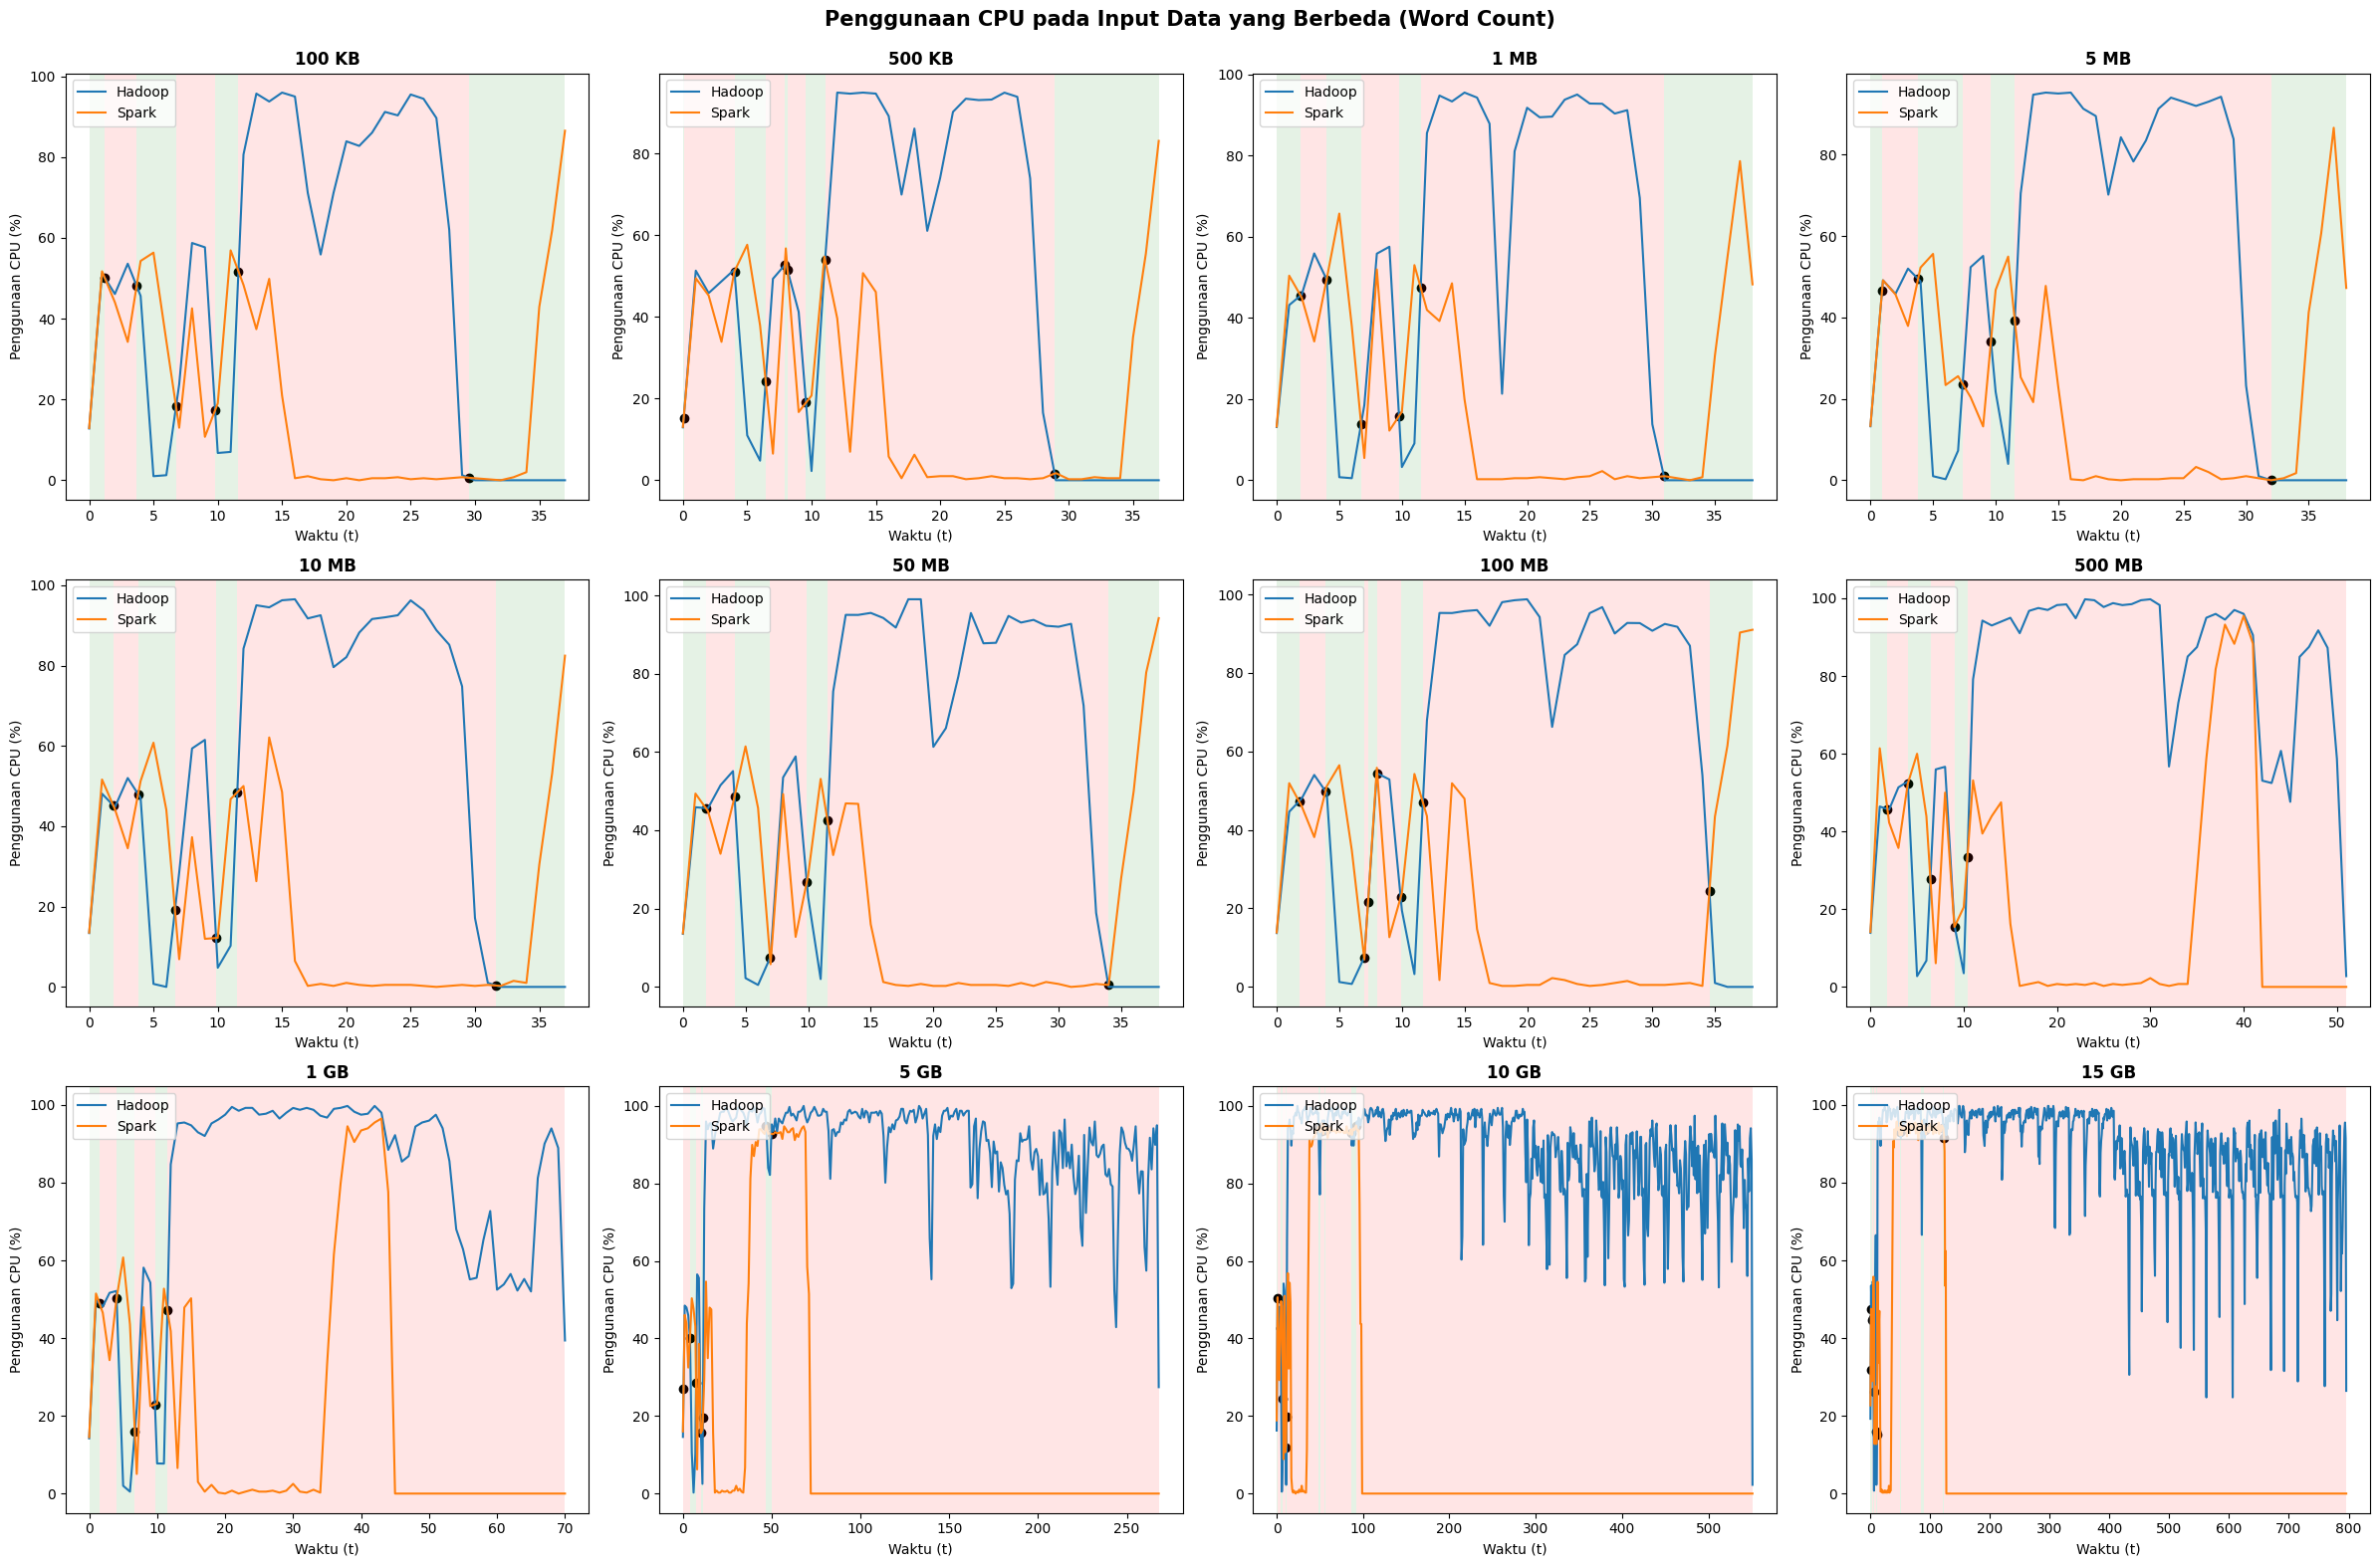
\includegraphics[height=0.6\linewidth]{figures/ch04/4-penggunaan-cpu-all-wordcount.png}
    \caption{Penggunaan CPU (\textit{Word Count})}
    \label{fig:4-penggunaan-cpu-all-wordcount}
\end{figure}
\end{landscape}

Gambar \ref{fig:4-state-sort} dan \ref{fig:4-state-wordcount} menyajikan \textit{bar chart} yang menggambarkan perbandingan persentase \textit{state} antara utilisasi Hadoop dan Spark untuk beban kerja \textit{sort} dan \textit{word count} pada berbagai ukuran data. \textit{State} $U_s$ merepresentasikan \textit{Utilization Spark} (Utilisasi Spark) dan \textit{state} $U_h$ merepresentasikan \textit{Utilization Hadoop} (Utilisasi Hadoop). Utilisasi yang dimaksud pada bagian ini adalah penggunaan CPU oleh Hadoop atau Spark.

Pada Gambar \ref{fig:4-state-sort}, secara konsisten $U_h > U_s$ memiliki nilai yang lebih tinggi dibandingkan dengan $U_h < U_s$. Hal ini berarti Hadoop memiliki penggunaan CPU yang lebih tinggi dan lebih banyak dari pada Spark. Contohnya, pada input data 100 KB, penggunaan CPU yang digunakan oleh Hadoop lebih tinggi selama 21.7 detik apabila dibandingkan dengan Spark hanya 15.3 detik. Begitu juga dengan input data yang lain. Hal yang menarik dari data ini adalah ketika input data 100 KB - 500 MB, perbandingan \textit{state} $U_h$ dan $U_s$ tidak berbeda jauh. Ketika input data diperbesar, nilai $U_h < U_s$ akan perlahan naik. Namun, gap dengan $U_h > U_s$ akan semakin membesar.

Selanjutnya, Gambar \ref{fig:4-state-wordcount} menampilkan perbandingan \textit{state} pada beban kerja \textit{word count}. Berbeda dengan \textit{sort}, beban kerja \textit{word count} menghasilkan \textit{state} $U_h > U_s$ dan $U_h < U_s$ yang lebih bervariasi, misalnya \textit{state} $U_h < U_s$ nilainya naik dan turun tidak bergantung dengan input data. Namun, nilai pada \textit{state} $U_h > U_s$ cenderung naik jika input data bertambah. Pada input data 15 GB, \textit{state} $U_h > U_s$ memiliki nilai 783.06 detik dan \textit{state} $U_h < U_s$ 12.94 detik. Hal ini menandakan bahwa kondisi CPU pada Hadoop lebih tinggi daripada Spark itu lebih banyak daripada kebalikannya. 

\begin{landscape}
\begin{figure}[h]
    \centering
    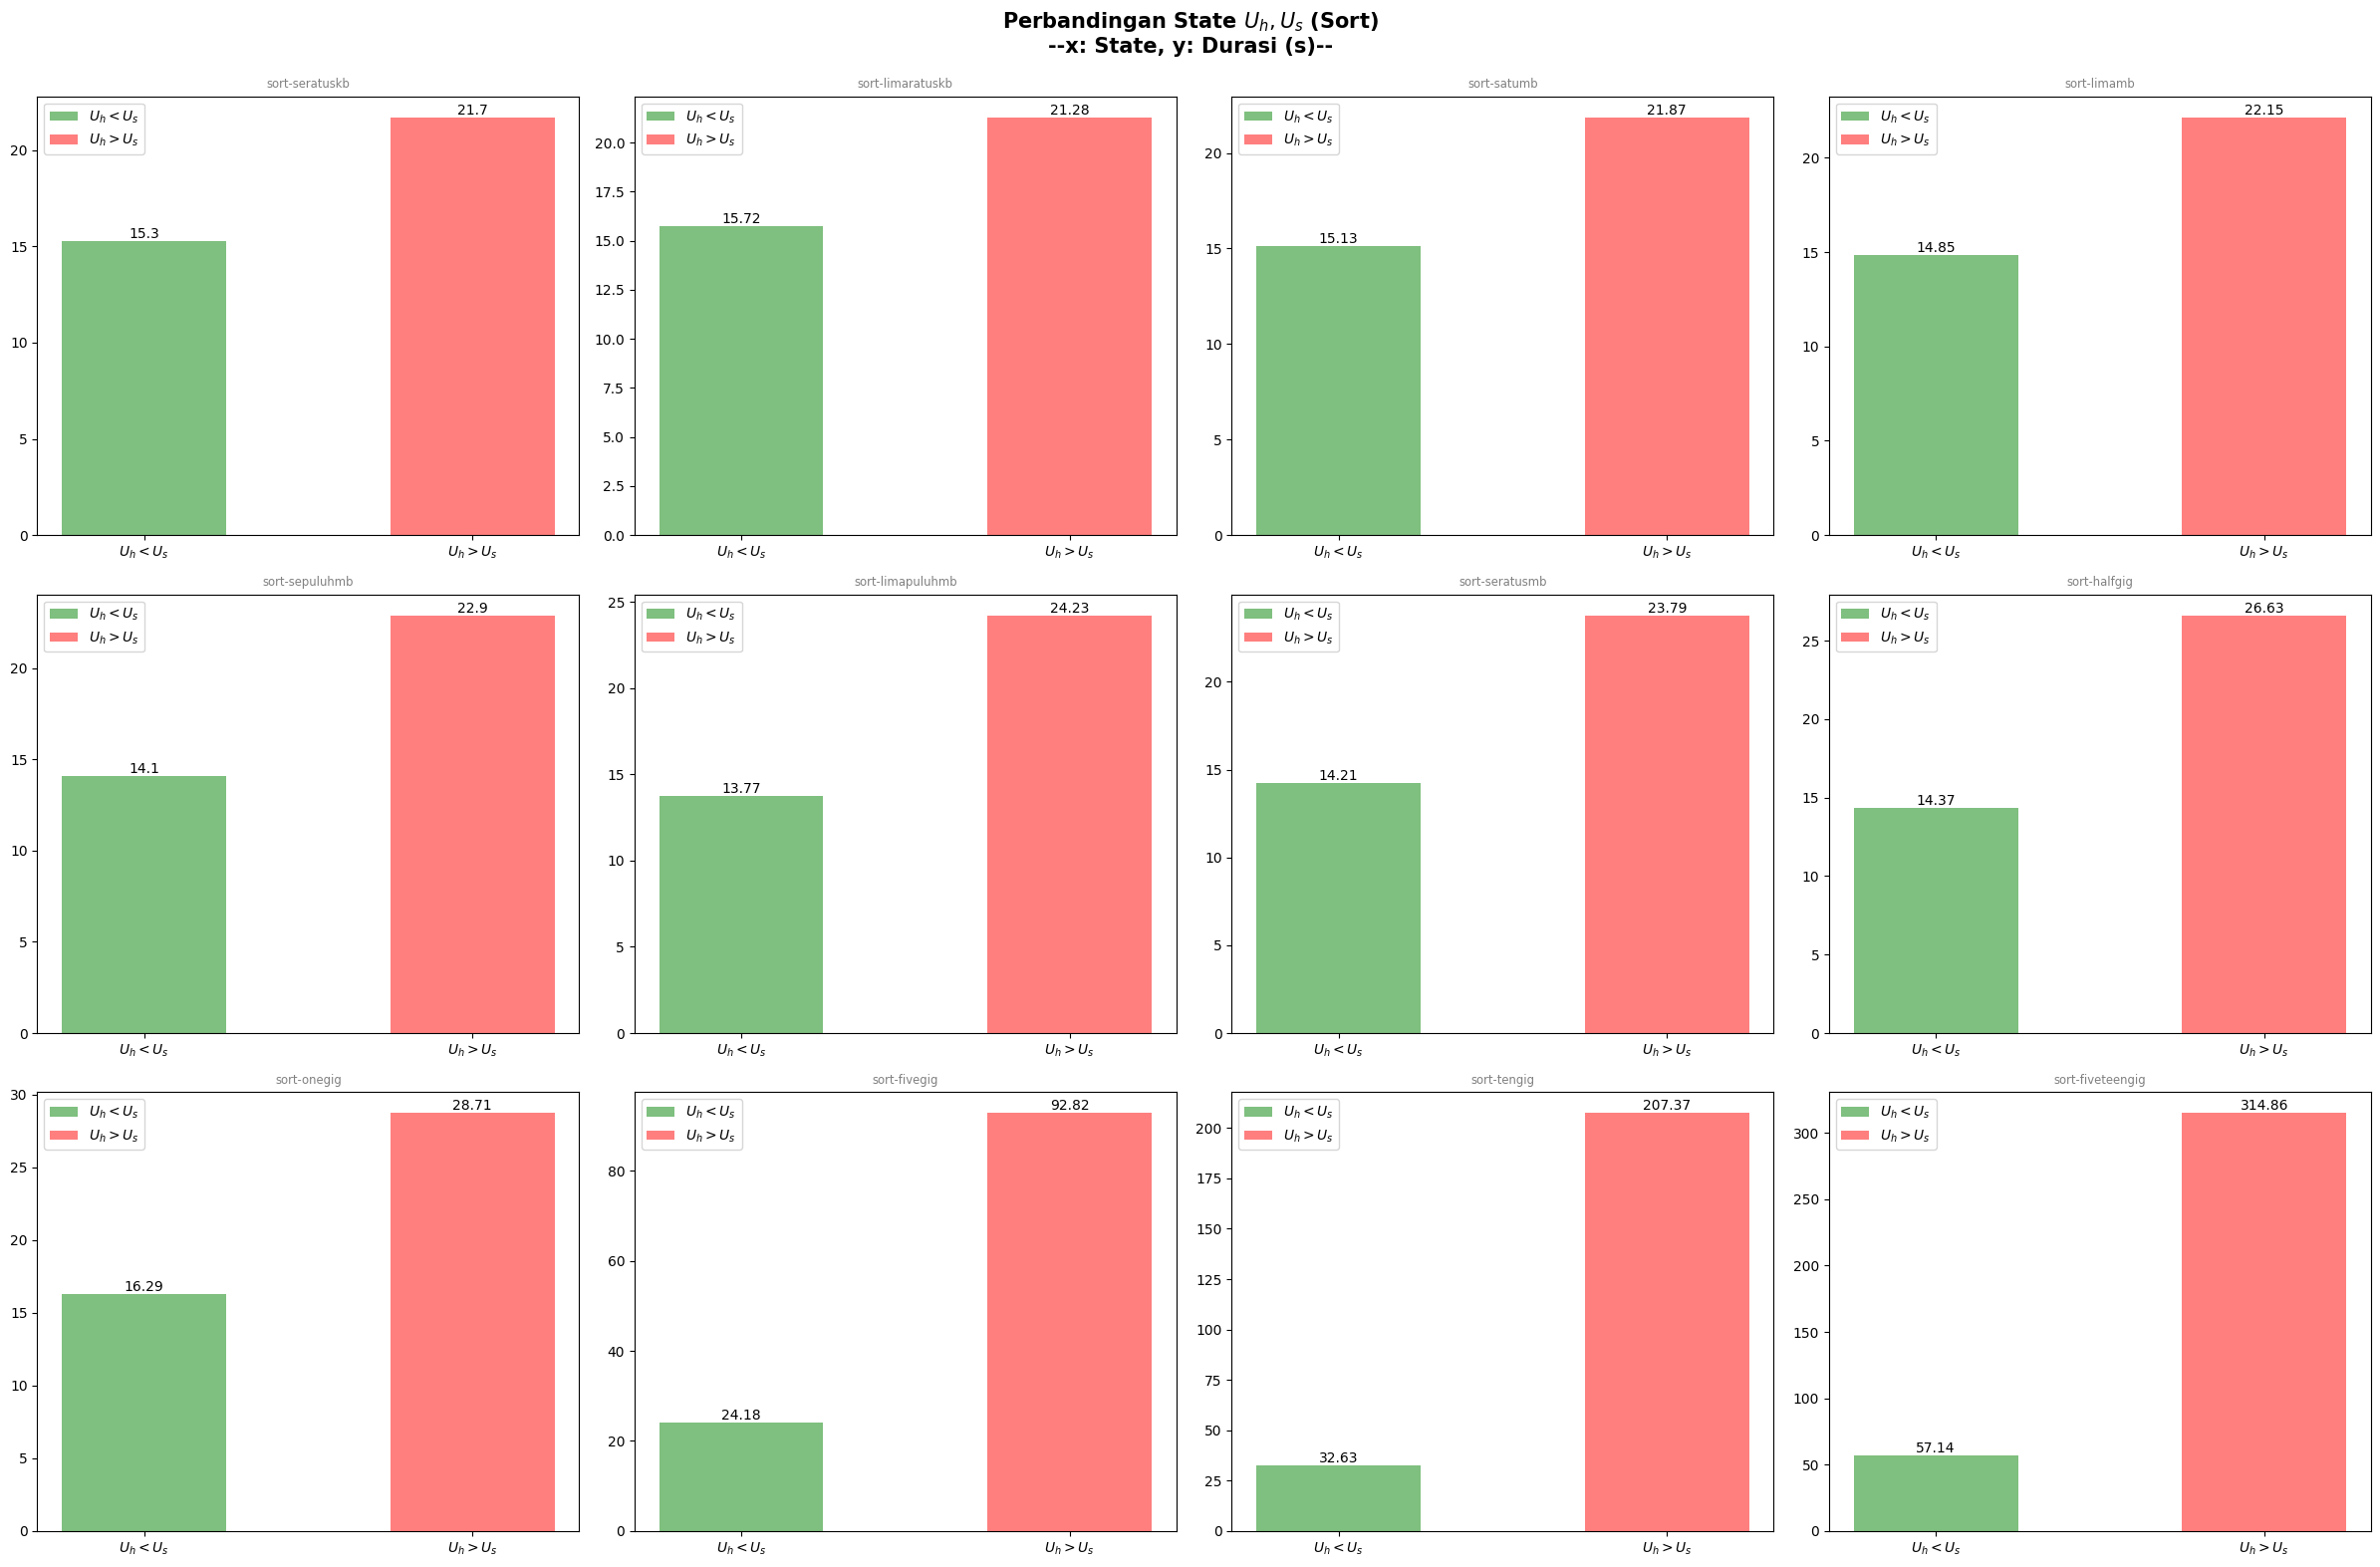
\includegraphics[height=0.6\linewidth]{figures/ch04/4-state-sort.png}
    \caption{Perbandingan \textit{State (Sort)}}
    \label{fig:4-state-sort}
\end{figure}
\end{landscape}

\begin{landscape}
\begin{figure}[h]
    \centering
    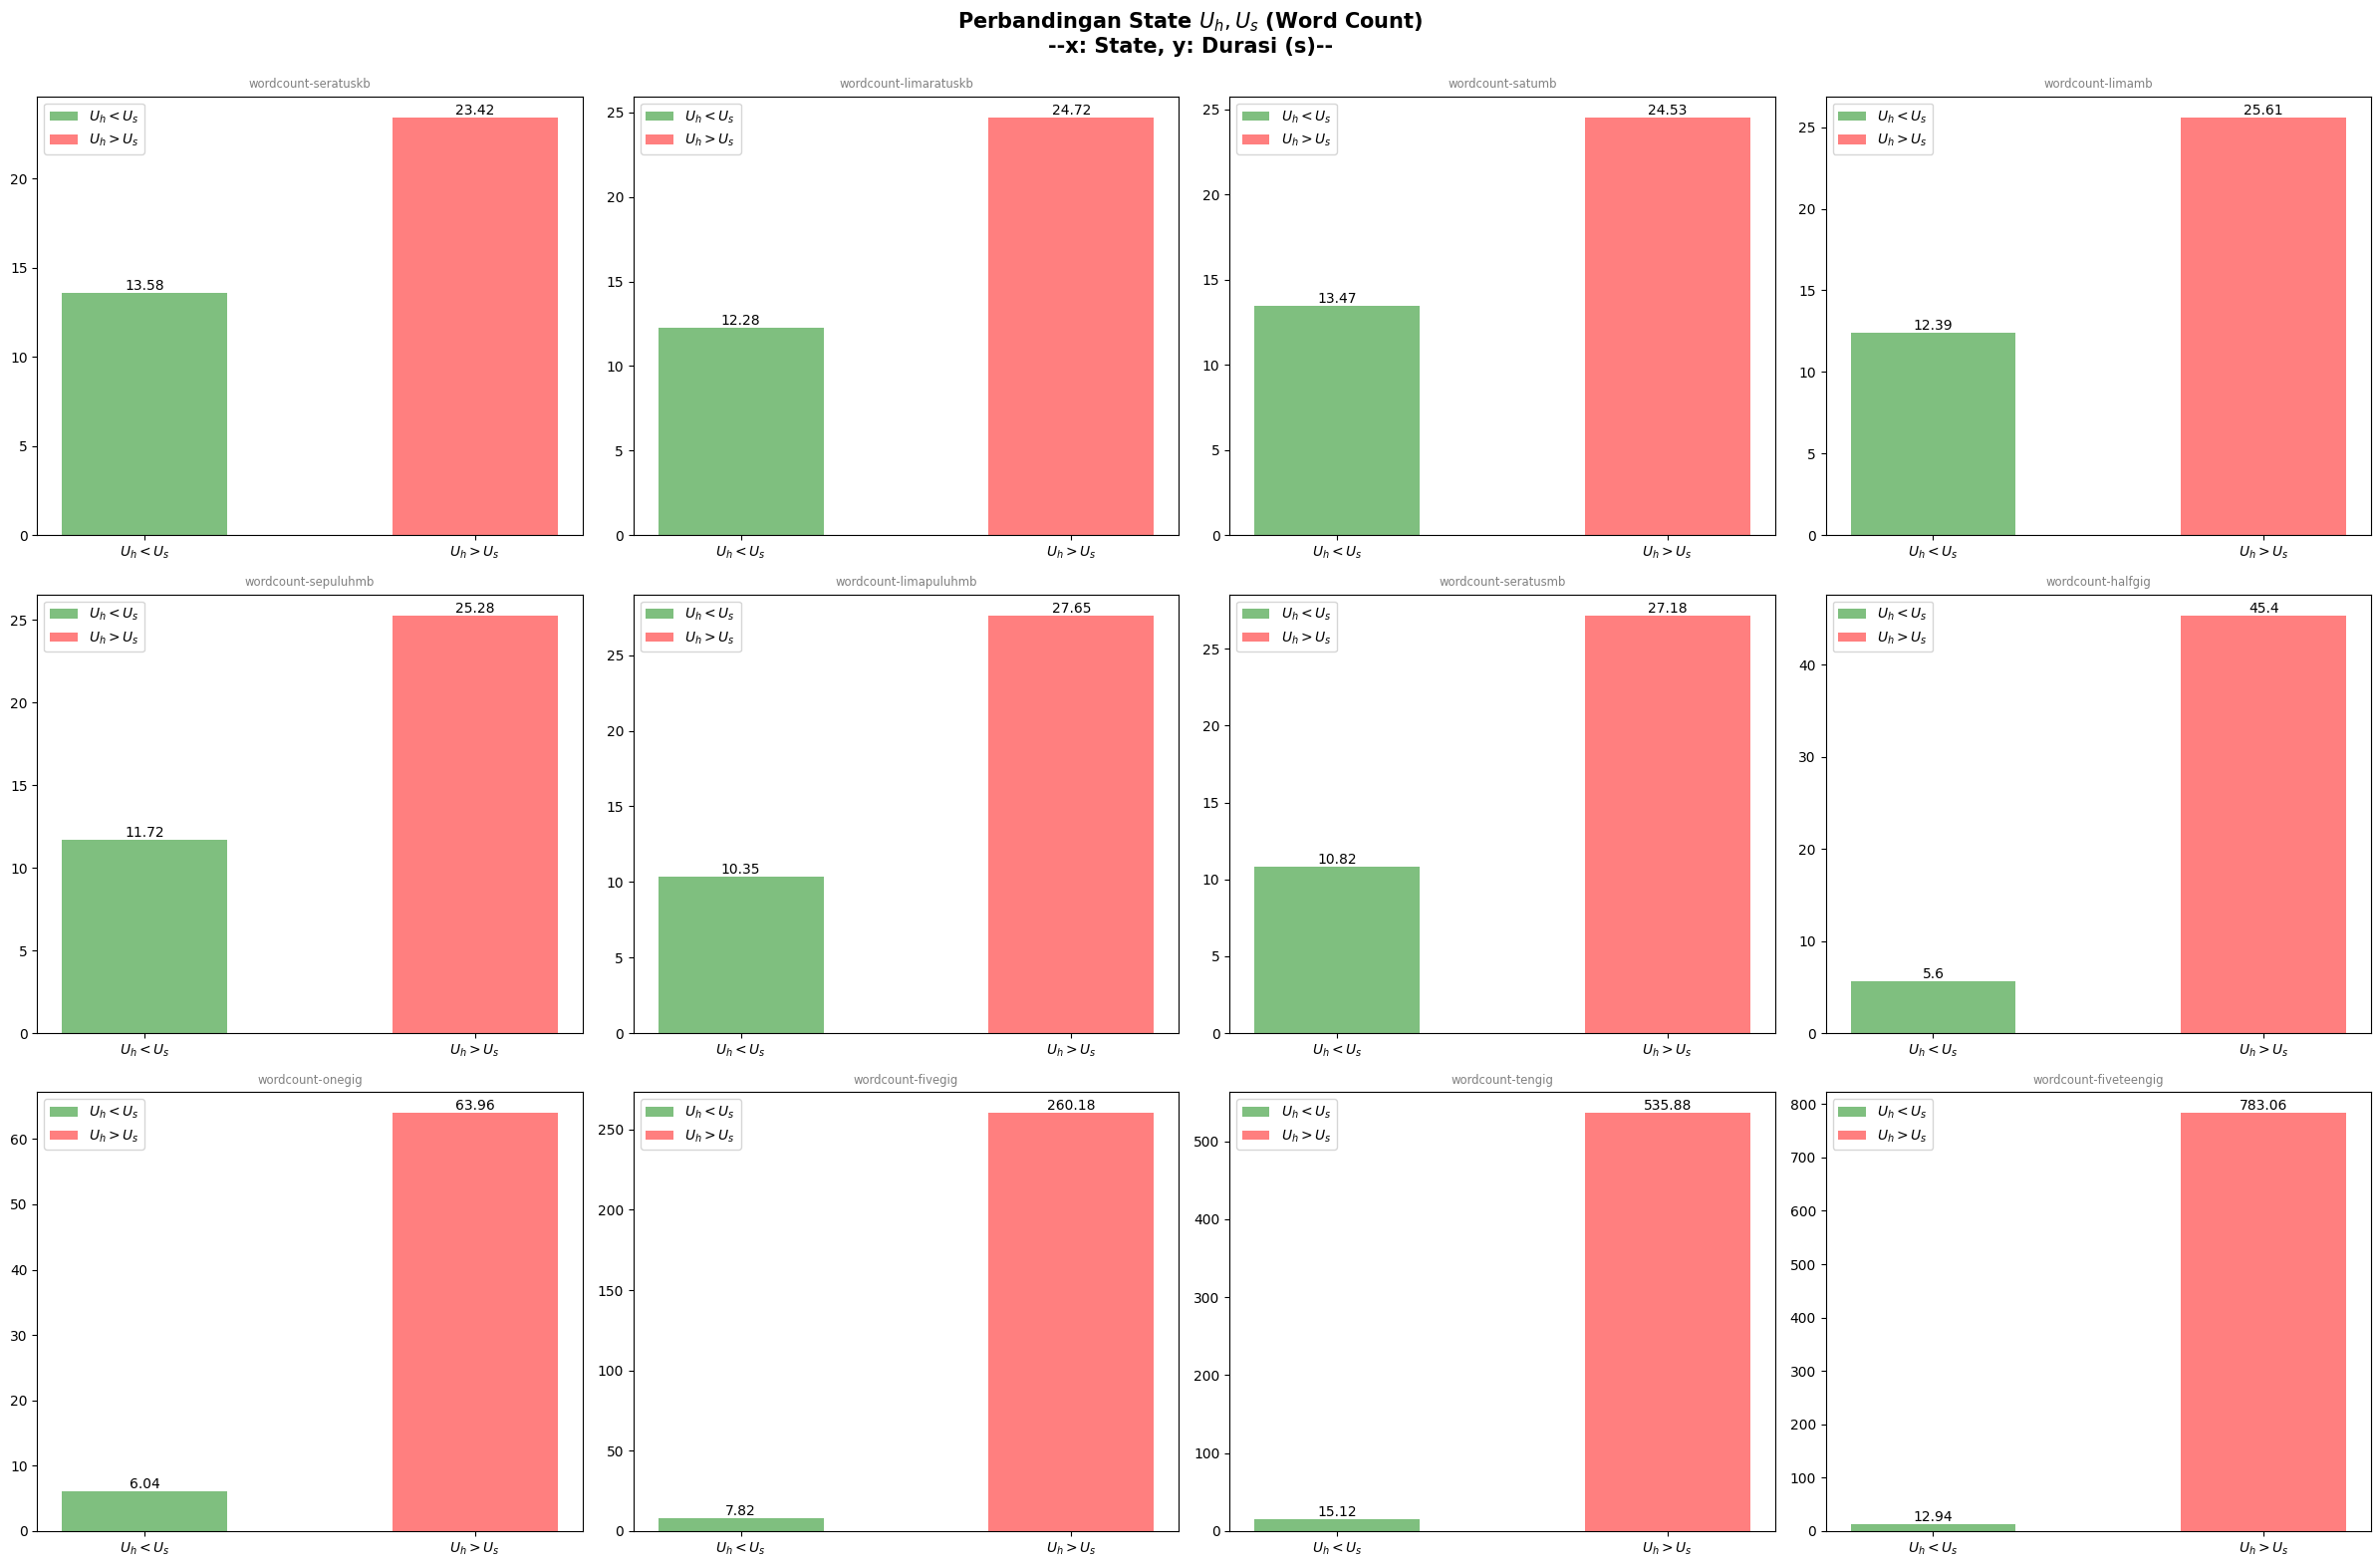
\includegraphics[height=0.6\linewidth]{figures/ch04/4-state-wordcount.png}
    \caption{Perbandingan \textit{State  (Word Count)}}
    \label{fig:4-state-wordcount}
\end{figure}
\end{landscape}

\newpage
\subsection{Utilisasi Sistem}
Utilisasi sistem secara lengkap dapat dilihat pada Lampiran \ref{appendix:G} untuk beban kerja \textit{sort} dan Lampiran \ref{appendix:H} untuk beban kerja \textit{word count}. Setiap gambar akan terdiri dari dua baris dan tiga kolom. Baris pertama berisi visualisasi utilisasi sistem untuk Hadoop dan baris keuda berisi visualisasi untuk Spark. Setiap baris berisi tiga utilisasi sistem, yaitu 
\begin{enumerate}
	\item Penggunaan CPU (\%)
	\item \textit{Disk} I/O (MB)
	\item Memori (GB)
\end{enumerate}

Berdasarkan analisis pola penggunaan CPU pada tahap sebelumnya yang menunjukkan bahwa penggunaan CPU Hadoop dan Spark memiliki polanya masing-masing, maka pada pada tahap ini hanya akan ditampilkan utilisasi sistem pada input data terkecil (100 KB) dan input data terbesar (15 GB). 

\begin{figure}[h]
    \centering
    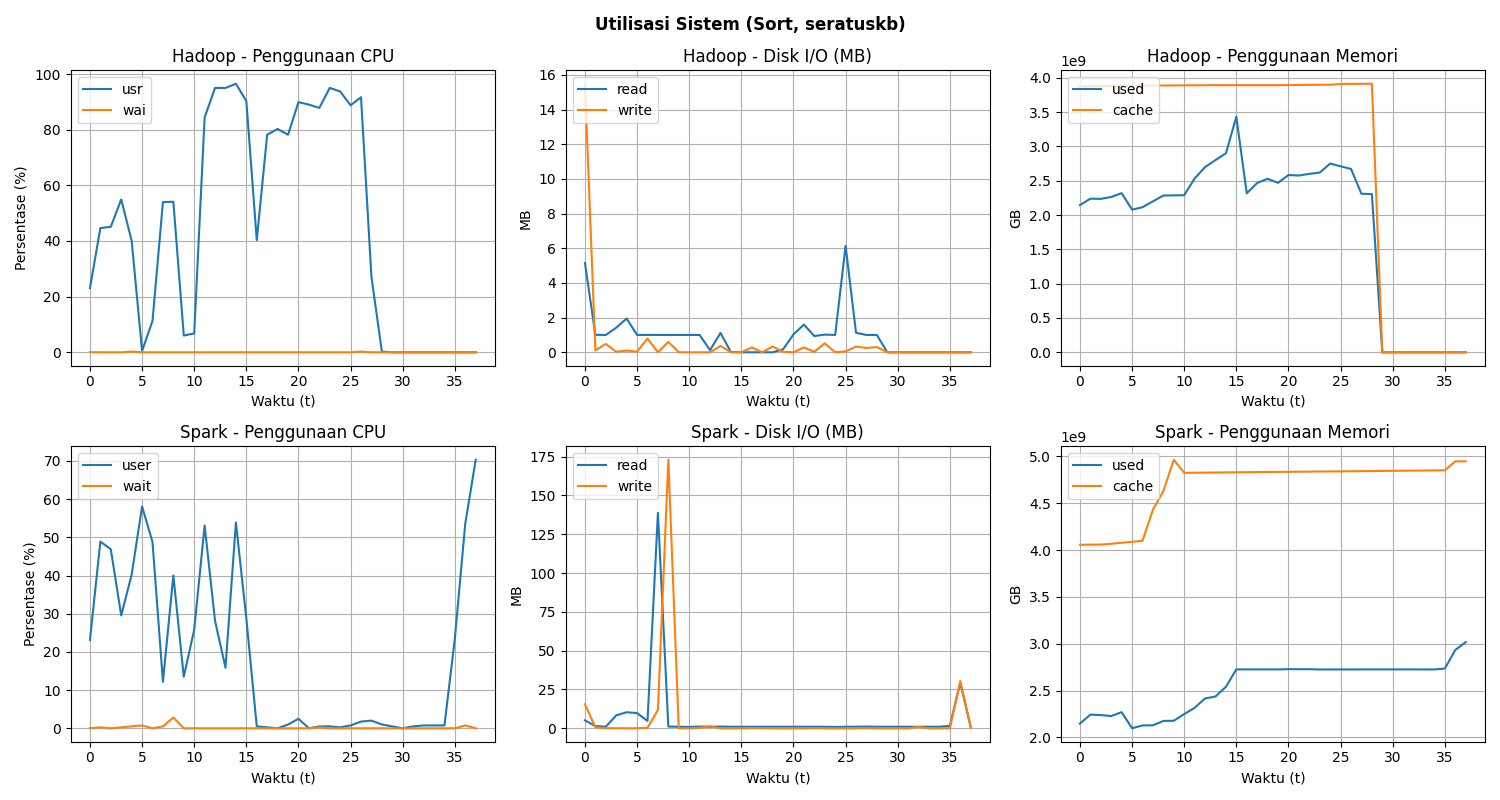
\includegraphics[width=1\textwidth]{figures/ch04/5-util-sistem-sort-seratuskb}
    \caption{Utilisasi Sistem (\textit{Sort}) pada Input Data 100 KB}
    \label{fig:5-util-sistem-sort-seratuskb}
\end{figure}

Pada beban kerja \textit{sort} dan input data sebesar 100 KB (seperti yang ditunjukkan Gambar \ref{fig:5-util-sistem-sort-seratuskb}), Hadoop memiliki penggunaan CPU yang lebih tinggi, yaitu hampir menyentuh 100\%. Sedangkan, pada Spark, penggunaan CPU tertinggi sekitar 70\%. Selanjutnya, ditinjau dari \textit{disk I/O}, aktivitas baca (\textit{read}) dan tulis (\textit{write}) pada Hadoop cenderung lebih sering namun memiliki kecepatan yang lebih lambat dibandingkan dengan Spark. Spark memiliki aktivitas baca tulis yang lebih tinggi, yaitu 140 MB untuk baca dan 175 MB untuk tulis. Kemudian, jika ditinjau dari penggunaan memori, Hadoop dan Spark memiliki penggunaan memori yang tidak berbeda jauh, yaitu sekitar 2 GB-3,5 GB. 

\begin{figure}[h]
    \centering
    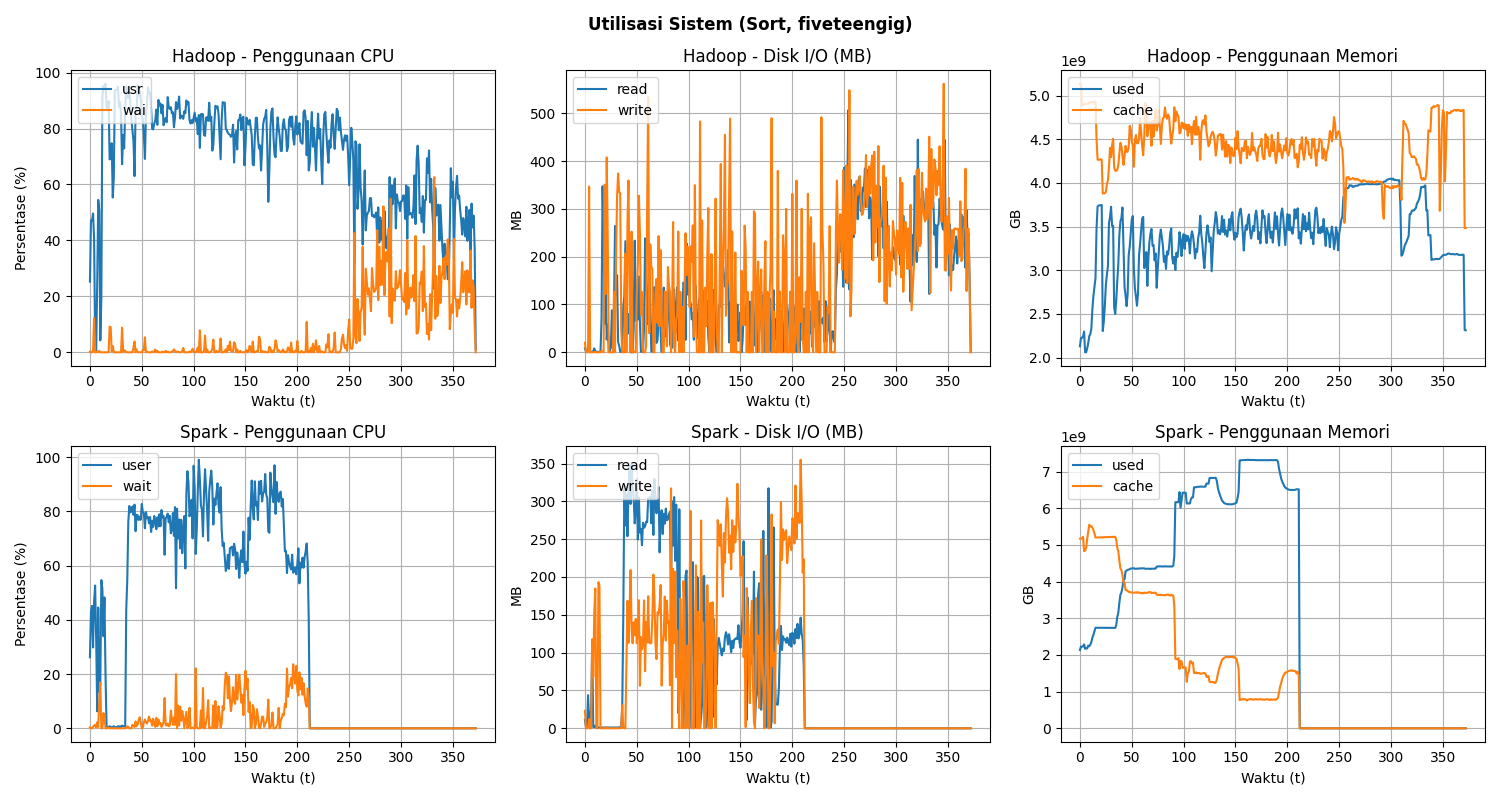
\includegraphics[width=1\textwidth]{figures/ch04/5-util-sistem-sort-fiveteengig}
    \caption{Utilisasi Sistem (\textit{Sort}) pada Input Data 15 GB}
    \label{fig:5-util-sistem-sort-fiveteengig}
\end{figure}

Pada beban kerja \textit{sort} dan input data yang lebih besar, yaitu 15 GB (seperti yang ditunjukkan pada Gambar \ref{fig:5-util-sistem-sort-fiveteengig}), utilisasi sistem pada Hadoop dan Spark lebih terlihat jelas perbedaannya. Jika dilihat pada penggunaan CPU, Hadoop membutuhkan waktu penggunaan CPU yang lebih lama, yaitu sekitar 370 detik, dimana Spark hanya membutuhkan waktu sekitar 220 detik. Selanjutnya, Hadoop memiliki penggunaan CPU "\textit{user}" yang lebih stabil, jika dibandingkan dengan Spark yang naik turun secara konstan. Penggunaan CPU "\textit{wait}" akan naik ketika penggunaan CPU "\textit{user}" itu turun. Bergeser pada \textit{disk I/O}, Hadoop memiliki siklus baca tulis yang lebih intensif jika dibandingkan pada Spark. Selanjutnya, jika dilihat dari penggunaan memori, Spark lebih "rakus" akan memori. Hal ini ditandai dengan puncaknya membutuhkan memori sekitar 6-7 GB, dimana Hadoop hanya membutuhkan memori sekitar 3,5 GB.

\begin{figure}[h]
    \centering
    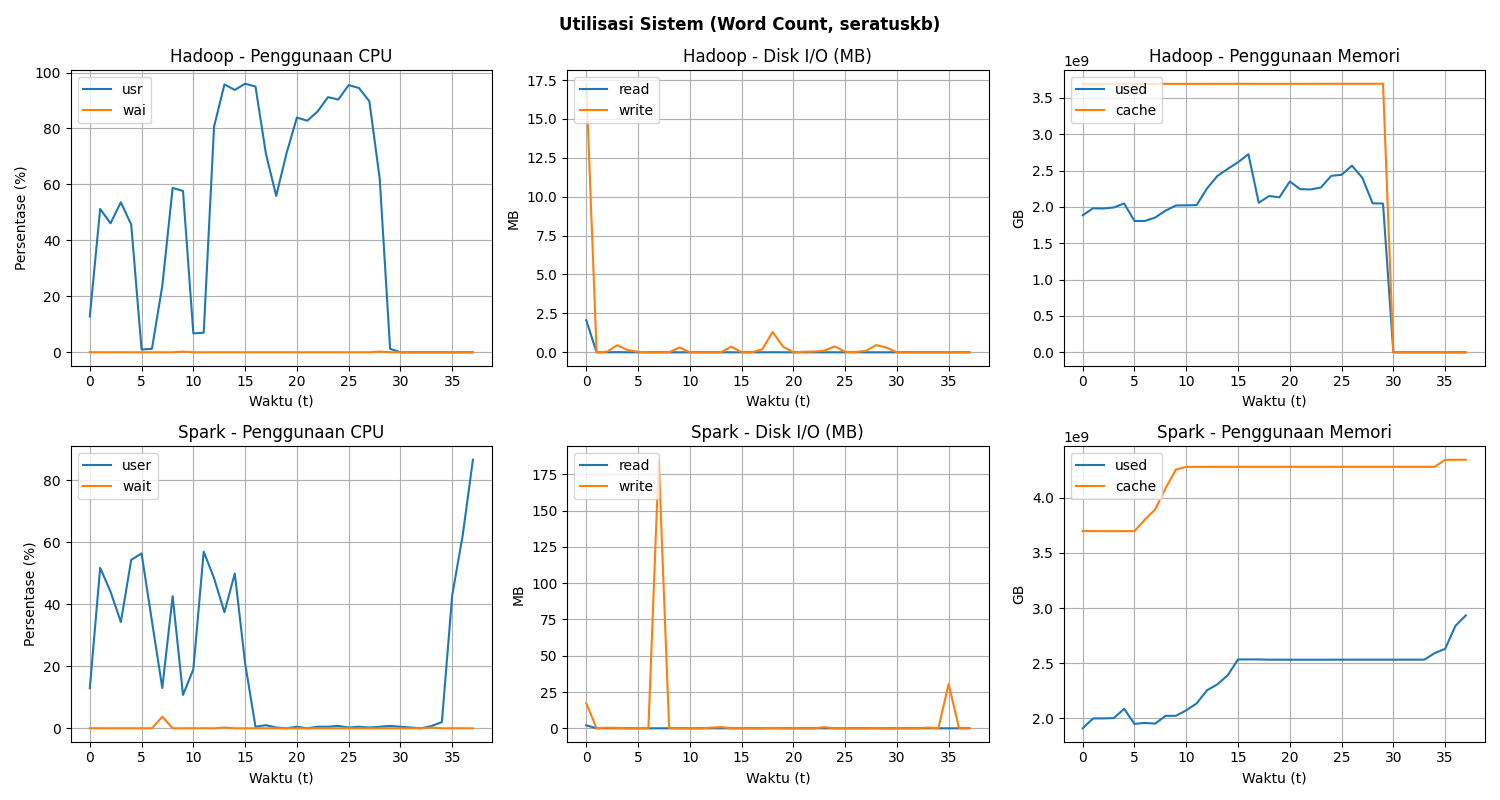
\includegraphics[width=1\textwidth]{figures/ch04/5-util-sistem-wordcount-seratuskb}
    \caption{Utilisasi Sistem (\textit{Word Count}) pada Input Data 100 KB}
    \label{fig:5-util-sistem-wordcount-seratuskb}
\end{figure}

Selanjutnya beban kerja \textit{word count}. Pada beban kerja \textit{word count} dengan input data 100 KB, pola yang didapatkan untuk penggunaan CPU, \textit{disk I/O}, dan penggunaan memori tidak berbeda jauh dengan beban kerja \textit{sort} dengan ukuran input data yang sama. 

\begin{figure}[h]
    \centering
    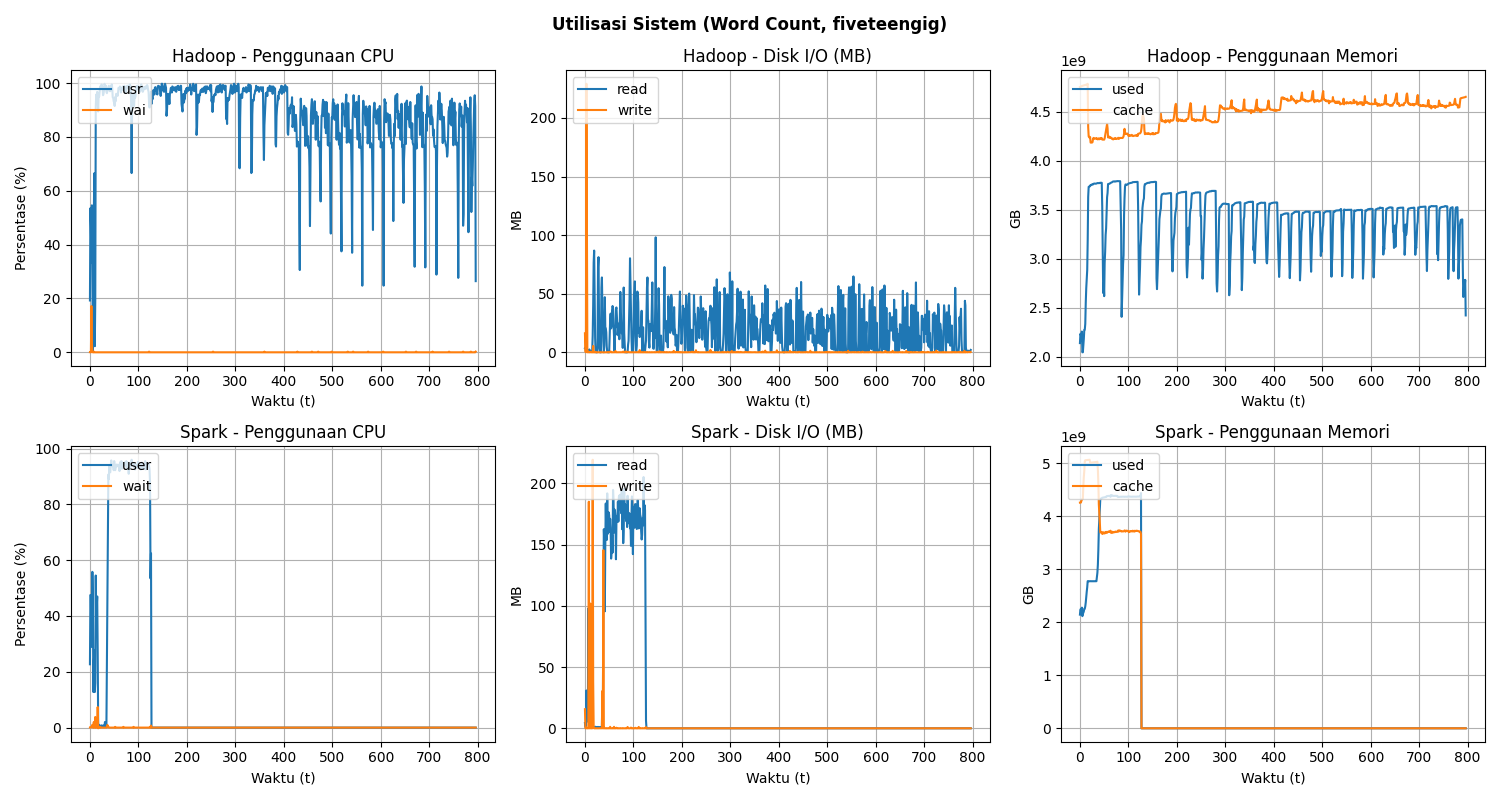
\includegraphics[width=1\textwidth]{figures/ch04/5-util-sistem-wordcount-fiveteengig}
    \caption{Utilisasi Sistem (\textit{Word Count}) pada Input Data 15 GB}
    \label{fig:5-util-sistem-wordcount-fiveteengig}
\end{figure}

Pada beban kerja \textit{word count} dan input data yang lebih besar, yaitu 15 GB (seperti yang ditunjukkan pada Gambar \ref{fig:5-util-sistem-wordcount-fiveteengig}), utilisasi sistem pada Hadoop dan Spark lebih terlihat jelas perbedaannya. Pada penggunaan CPU, Hadoop memiliki aktivitas penggunaan yang lebih tinggi dan lebih konstan sampai akhir waktu eksekusi. Hal ini berbeda dengan Spark yang hanya butuh waktu sekitar 150 detik saja dengan penggunaan CPU yang hanya 90\%. Selanjutnya, pada aktivitas baca tulis (\textit{disk I/O}), Hadoop memiliki aktivitas baca yang lebih intensif (sepanjang waktu eksekusi) dengan sedikit aktivitas tulis (pada awal waktu eksekusi). Aktivitas baca yang dilakukan oleh Hadoop berada pada ukuran 50-100 MB setiap waktunya. Pada Spark, aktivitas baca tersebut berukuran 150-200 MB. Kemudian, jika ditinjau melalui penggunaan memori, memori yang dibutuhkan Hadoop berkisar pada 2,5-3,7 GB. Pada Spark, memori yang dibutuhkan berkisar pada 2-4,5 GB.  

Hadoop menunjukkan aktivitas \textit{Disk} I/O yang jauh lebih tinggi dibandingkan dengan Spark, terutama pada beban kerja \textit{sort}. Grafik \textit{Disk} I/O Hadoop menunjukkan lonjakan aktivitas baca dan tulis yang signifikan sepanjang waktu eksekusi. Hal ini sesuai dengan pendekatan berbasis disk Hadoop yang membutuhkan pembacaan dan penulisan data ke \textit{disk} secara intensif. Sebaliknya, Spark, dengan arsitektur in-memory, meminimalkan operasi \textit{Disk} I/O. Grafik \textit{Disk} I/O Spark menunjukkan aktivitas yang jauh lebih rendah dan stabil, yang berkontribusi pada peningkatan performanya.

Spark menunjukkan penggunaan memori yang lebih tinggi dan stabil dibandingkan dengan Hadoop, terutama pada beban kerja \textit{sort}. Grafik penggunaan memori Spark menunjukkan garis yang cenderung mendatar pada tingkat utilisasi yang tinggi, menunjukkan bahwa Spark menyimpan data dalam RAM untuk akses yang lebih cepat dan pemrosesan yang efisien. Penggunaan memori Hadoop lebih rendah dan fluktuatif, menunjukkan bahwa Hadoop tidak memanfaatkan memori secara optimal. 

Analisis pemantauan sistem menegaskan keunggulan Spark dalam hal efisiensi dan optimasi penggunaan sumber daya komputasi dibandingkan dengan Hadoop. Spark mampu memaksimalkan penggunaan CPU, meminimalkan operasi \textit{Disk} I/O, dan memanfaatkan memori secara efisien, yang berkontribusi pada performa dan skalabilitas yang lebih baik dalam tugas-tugas pemrosesan data besar.
